\documentclass[12pt,a4paper]{article}
\usepackage[a4paper, total={7in, 8in}]{geometry}

\usepackage[utf8]{inputenc}
\usepackage[T1]{fontenc}
\usepackage[export]{adjustbox}
\usepackage[french]{babel}
\usepackage{graphicx}
\usepackage{eso-pic}
\usepackage{transparent}
\usepackage[export]{adjustbox}
\usepackage{hyperref} \hypersetup{colorlinks, citecolor=black, filecolor=black, linkcolor=black, urlcolor=black,}
\usepackage[nonumberlist]{glossaries}
\usepackage{glossaries}
\usepackage{imakeidx}
\usepackage{float}

% 1 : Logo ulb en fond
\newcommand\BackgroundPic{%
    \put(0,-47){%
        \parbox[b][\paperheight]{\paperwidth}{%
            \vfill
            \centering
            {\transparent{0.09}
\includegraphics[width=1.17 \textwidth]{Fondulb.jpg}}%
            \vfill
        }
    }
}





% Glossaire
\newglossaryentry{Tower Defense}
{
	name=Tower Defense,
    description={Jeu de stratégie où le but est de défendre la zone d'un \gls{joueur} contre des vagues  successives d'\glspl{ennemi}\index{ennemi} en construisant et en améliorant progressivement ses tours.}
}
\newglossaryentry{joueur}
{
	name=joueur,
    description={Personnage fictif du jeux qu'incarne l'\gls{utilisateur}}
}

\newglossaryentry{utilisateur}
{
	name=utilisateur,
    description={Personnage réel qui joue à Meatwars: Revenge of the Falling Vegan}
}

\newglossaryentry{compte}
{
	name=compte,
    description={Contient toutes les données de l'\gls{utilisateur}}
}

\newglossaryentry{serveur}
{
	name=serveur,
    description={Programme qui réceptionne les connections des \glspl{client}. Il a les données de tous les \glspl{utilisateur}}
}

\newglossaryentry{client}
{
	name=client,
    description={Programme que l'\gls{utilisateur} lance pour se connecter au \gls{serveur}. Il permet à l'\gls{utilisateur} de jouer au jeu via le terminal ou l'interface graphique}
}

\newglossaryentry{ennemi}
{
	name=ennemi,
	description={Personnage fictif qui apparaît avec intervalle régulier dans une vague qui a un certain niveau de vie.}
}

\newglossaryentry{argent}
{
	name=argent,
	description = {Monnaie qui permet au \gsl{joueur} de s'acheter des tours pour permettre de résister aux vagues d'\glspl{ennemi}.}
}

\newglossaryentry{tour}
{
	name=tour,
	description={Objet de défense permettant à un joueur de contrer les vagues d'\glspl{ennemi}, à  chaque \gls{ennemi} détruit le \gls{joueur} gagne de la \gls{argent}.}
}

\newglossaryentry{map}
{
	name= map,
	description={Espace représentant le plateau de jeu avec lequel les joueurs pourront avoir des interactions(placer des tours sur les partie délimité par des \# et montreras aussi le déplacement des \glspl{ennemi} selon des chemins prédéfinies.}
}

\newglossaryentry{supporter}{
    name= supporter,
    description={Personnage fictif que l'\gls{utilisateur} qui ne peut peut jouer une partie mais peut intervenir en donnant de l'\gls{argent} à un \gls{joueur} ou plusieurs.}
}
\newglossaryentry{thread}
{
    name = thread,
    description = {Un processus possédant plusieurs tâches qui s'exécutent de manière quasi-simultané. }
}
\newglossaryentry{pseudo}{
    name = pseudo,
    description = {Un pseudo est un nom fictif crée par un \gls{joueur}.}
    
}
\newglossaryentry{tourelle}{
    name = tourelle,
    description = {Une tourelle dans le cadre de ce jeu, est un item défensive placé par le \gls{joueur} pour se défendre contre les vagues d'ennemis.}
    
}
\newglossaryentry{qt}{
    name = qt,
    description = {Librairie c++ utilisée dans ce projet pour la réalisation de la partie graphique.}
    
}
\makeglossaries
\setglossarysection{subsection}


\makeindex
\indexsetup{level=\chapter}
% Pour ajouter un mot à l'index: "\index{mot}"



\begin{document}
\AddToShipoutPicture*{\BackgroundPic}

\begin{titlepage}
\begin{center}
\vspace*{-1.5cm}

\includegraphics[width=8cm]{ulb.pdf}
\vspace{6cm}

\par{\huge \textbf{SRD: Tower Defense}}\bigbreak
\bigbreak
\par{\huge \textbf{\textit{{Meat war: Rise of the fallen vegan}}}}
\vspace{2cm}
\par{\large [Cours: INFO-F-209]}
\vspace{2cm}

\par \hrulefill \par
\vspace{1cm}
\bsc{Jacobs} Alexandre 
\bsc{\&}
\bsc{Innocent} Antoine
\bsc{\&}
\bsc{André} Bob
\bsc{\&}
\bsc{Vangeem} Nicolas
\bsc{\&}
\bsc{Roos} Kim
\bsc{\&}
\bsc{Paquet} Michael
\bsc{\&}
\bsc{Singh} Sundeep
{\emph \\BA2 Informatique}
\vspace{0.7cm}
\par \hrulefill \par

\vspace{2cm}
\par Mars 2017

\end{center}
\end{titlepage}
\newpage
\tableofcontents
\newpage

\section{Introduction}
\subsection{But du projet}
 Notre projet consiste en une réalisation d'un \index{\gls{Tower Defense}} qui sera jouable en réseau sous Linux. Il est aussi de permettre aux étudiants de mettre en pratique les différents concept vus dans les cours de système d'exploitation et d' analyse et méthodologie informatiques. De plus, le respect de conventions de codage, du paradigme orienté-objet et l'analyse UML faites seront un aspect essentiel à la réalisation de notre projet.  


Ce document joue le rôle du document de spécification des besoins, SRD (System requirement Document) pour le projet INFO-F209 : "Meat war: Rise of the falling vegan".
	Ces exigences portent sur un travail de groupe (8 personnes) codé majoritairement en C++ avec une section C pour le \gls{serveur} \index{serveur}. Le produit final est donc un jeu de type \gls{Tower Defense} \index{Tower Defense} multijoueur en réseau.
Ce jeu n'ayant aucun but lucratif, nous considérons le \index{\gls{client}} principal comme étant le \gls{joueur}\index{joueur} du jeux en question.
Ainsi, ce document présente des spécifications propres à l'\gls{utilisateur}\index{utilisateur} et propre au système. Celui-ci va également mettre en avant la communication \gls{client} \index{client}/ \gls{serveur} \index{serveur} afin de bien mettre en place l'aspect multijoueur réseau du produit. 


 Ce document ne varie pas en fonction des différentes architectures ou systèmes d'exploitation.

\subsection{Présentation du jeu}
 Le nom de notre projet est "Meat war: Rise of the fallen vegan".
Lors d'une création de \gls{compte}\index{compte}, chaque \gls{utilisateur}\index{utilisateur} reçoit une certaine somme d' \glspl{argent} \index{argent} qui lui permettra d'acheter des tours \index{tours} lors des parties.
\noindent Lors de partie, chaque \gls{joueur}\index{joueur} se voit attribuer une partie de la \gls{map}\index{map}. Chaque \gls{joueur}\index{joueur} utilisant à sa guise la partie de la \gls{map}\index{map} lui ayant été attribué. Par ailleurs, les termes utilisé et lié au jeu ont été choisis en fonction du thème que nous sommes imposés.

% Glossaire
\glsaddall
\printglossary[numberedsection]

\subsection{Historique de document}

\begin{center}
\hspace*{0cm}
\begin{tabular}{|c|c|c|c|}
\hline
Versions & Auteur & Date & Modifications \\
\hline
3.0 & Équipe & 30-03-2017 &\textbf{Deadline pour la phase 3.}\\
2.8 & Sundeep & 27-03-2017 & Ajout diagramme d'activité menu.\\
2.7 & Sundeep & 27-03-2017 & Ajout diagramme d'activité inscription. \\
2.6 & Sundeep & 27-03-2017 & Ajout diagramme d'activité se connecter.\\
2.5 & Sundeep & 27-03-2017 & Ajout diagramme séquence du matchmaking.\\
2.4 & Sundeep & 27-03-2017 & Ajout Seq Diag de l'accès à une donnée.\\
2.3 & Sundeep & 27-03-2017 & Ajout descriptions des tous les modules.\\
2.2 & Sundeep & 27-03-2017 & Ajout diagramme de séquence en jeu.\\
2.1 & Sundeep & 27-03-2017 & Révision des uses case et descriptions\\
2.0 & Équipe & 05-03-2017 &\textbf{Deadline pour la phase 2}\\
1.5 & Alexandre & 05-03-2017 & Mise à jour diagramme UML\\
1.4 & Alexandre & 28-02-2017 & Révision besoin système \& utilisateur.\\
1.3 & Alexandre & 28-02-2017 & Ajout de certains termes.\\
1.2 & Alexandre & 27-02-2017 & Modification de la section Introduction.\\
1.1 & Antoine \& Bob & 10-02-2016 & Correction suite à de la réunion du 06-02-2017. \\
1.0 & Équipe & 19-12-2016 & \textbf{Deadline pour la phase 1}\\
0.3 & Kim & 16-12-2016 & Ajout du glossaire et de l'index\\
0.2 & Équipe & 16-12-2016 & Ajout des besoins utilisateur et système\\
0.1 & Sundeep \& Michael & 10-12-2016 & Ajout des use cases et diagrammes d'activité au niveau utilisateur.\\
0.0 & Alexandre \& Antoine & 10-12-2016 & Création de la structure du document.\\
\hline
\end{tabular}
\end{center}


\newpage
\section{Besoins de l'utilisateur}

 Les besoins de l'\gls{utilisateur}\index{utilisateur} seront expliqués au travers de plusieurs graphes/explications, en voici ici un résumé.\\
Le but de l'application est de permettre à l'\gls{utilisateur}\index{utilisateur} de pouvoir jouer à un jeu de type \gls{Tower Defense} \index{Tower Defense}. Celui-ci sera disponible depuis un menu\index{menu} accessible après connexion et offrira au \gls{utilisateur}\index{utilisateur} plusieurs services. En effet, l'\gls{utilisateur}\index{utilisateur} devra se créer un \gls{compte}\index{compte} avant d'avoir accès au menu.\\
Il pourra alors consulter son profil\index{consulter son profil}.
Un classement\index{classement} sera également accessible et permettra de situer un \gls{joueur}\index{joueur} par rapport à un autre en fonction de leur score respectif.\\
Comme dit implicitement plus haut, l'\gls{utilisateur}\index{utilisateur} disposera d'une liste d'amis\index{liste d'amis} qui pourra modifier(ajouter, supprimer et accepter des demandes d'amis) et afficher sa liste d'amis.\\

 Le menu\index{menu} permettra bien évidemment à un \gls{utilisateur}\index{utilisateur} premièrement de se connecter à un \gls{compte}\index{compte} déjà existant ou de se créer un \gls{compte}\index{compte}, deuxièmement une fois l'\gls{utilisateur}\index{utilisateur} connecté, ce dernier pourra décider de démarrer une partie, donc de choisir un mode de jeu pour qui ouvrira un salon en attendant d'avoir le nombre requis de \glspl{joueur} afin de jouer une partie. Mode, et nombre de \glspl{joueur}\index{joueur} (au maximum de 4) seront spécifiés par le \gls{client} avant que celui-ci ne lance la partie\index{partie}. Il pourra aussi rejoindre une partie en tant que \gsl{supporter}\index{supporter}, afficher son profil et gérer ses amis. Une seule et unique carte sera cependant disponible.
 
\subsection{Exigences fonctionnelles}
Les besoins fonctionnels sont représentés par deux diagrammes uml.Ceux-ci sont repris ci-dessous et représentent une partie de l'application.Bien évidemment, ceux-ci sont accompagnés des post-conditions, pré-conditions...


\begin{figure}[H]

\begin{center}
    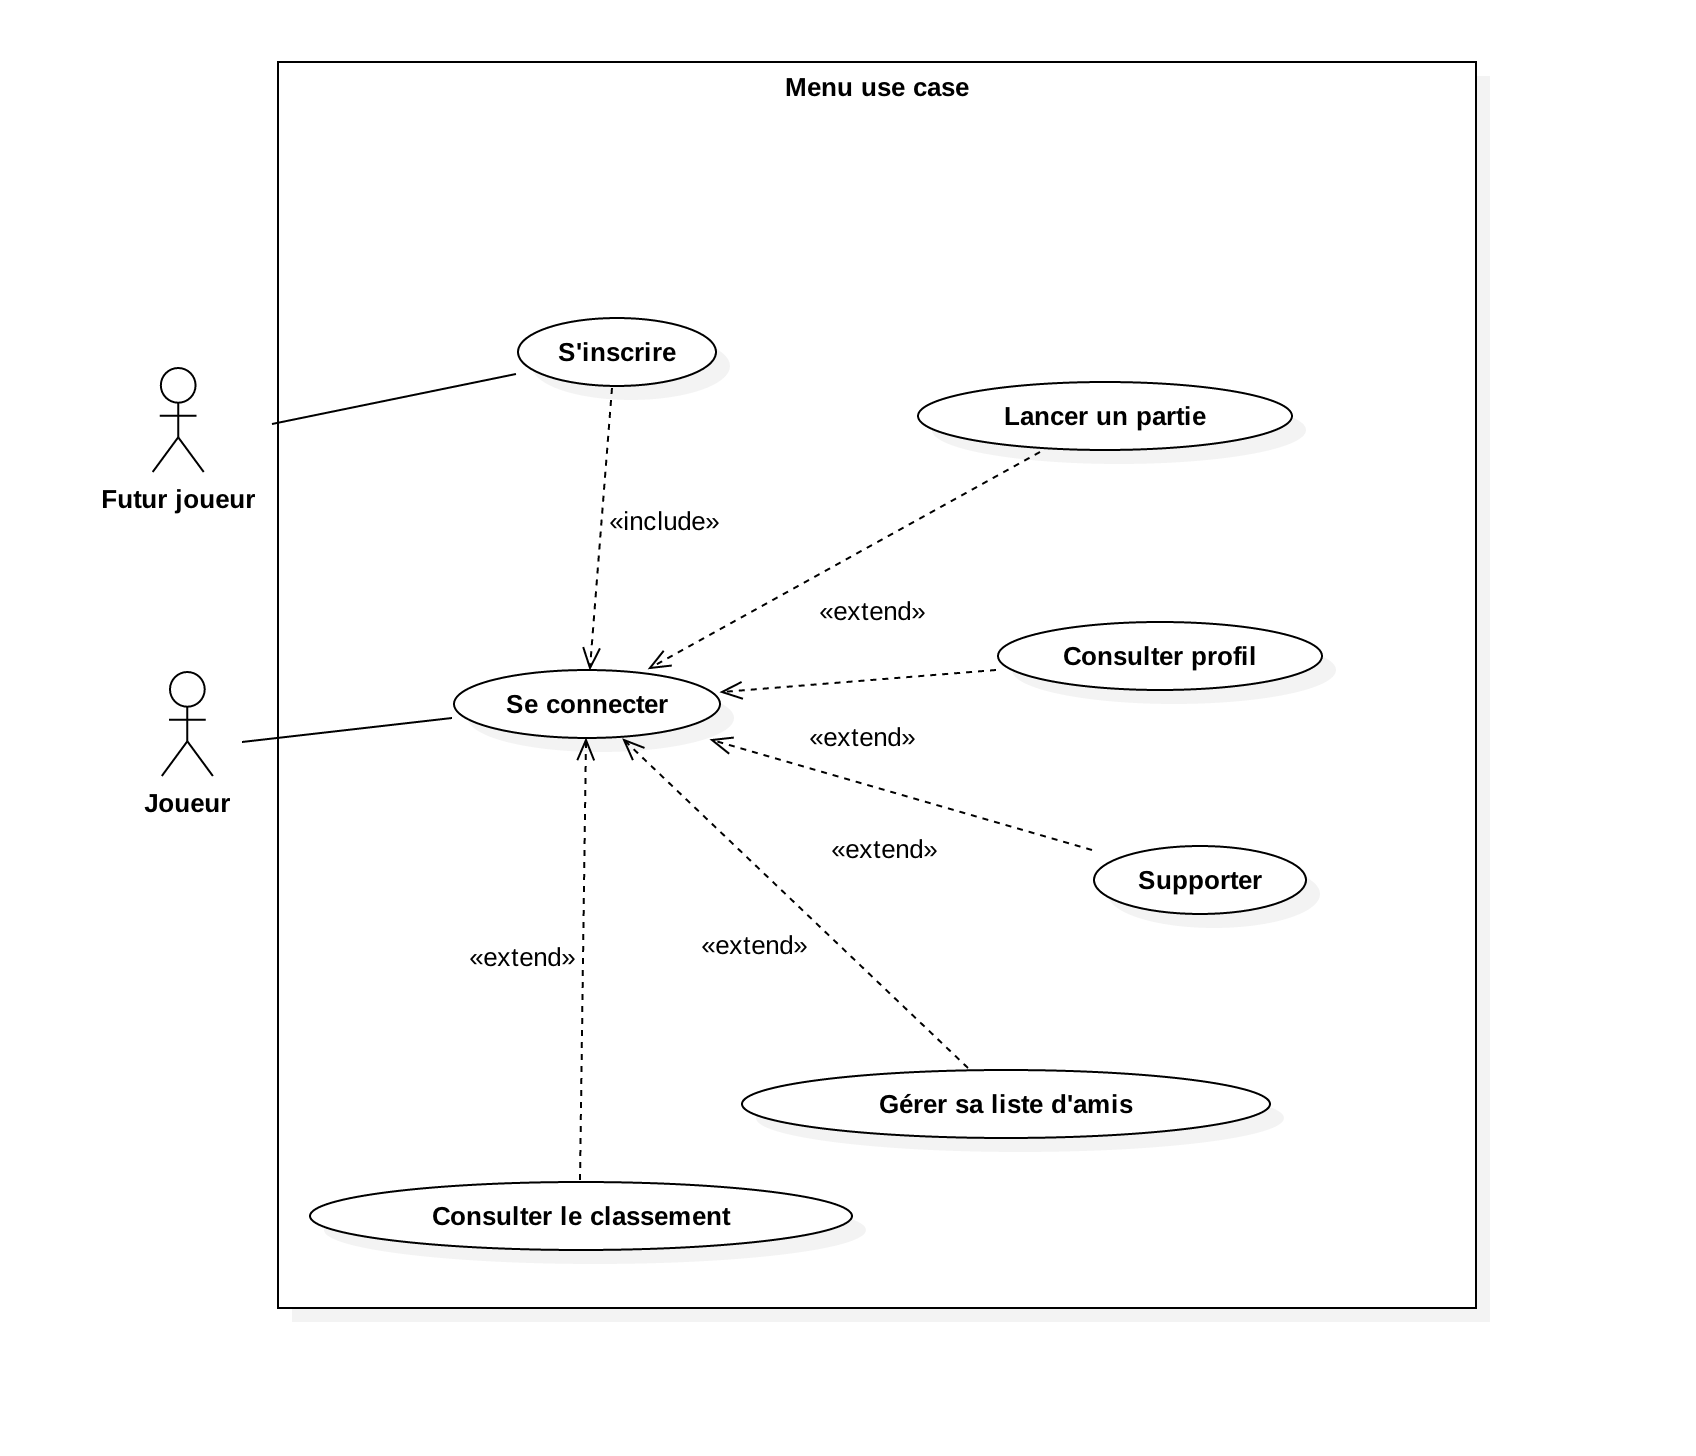
\includegraphics[height=12cm,width=16.45cm]{menu_use_case.png}
    \caption{Diagramme uml avant partie}   
  \label{fig:picture}
\end{center}
\end{figure}
\par
%\newpage
\begin{figure}[H]

\begin{center}
    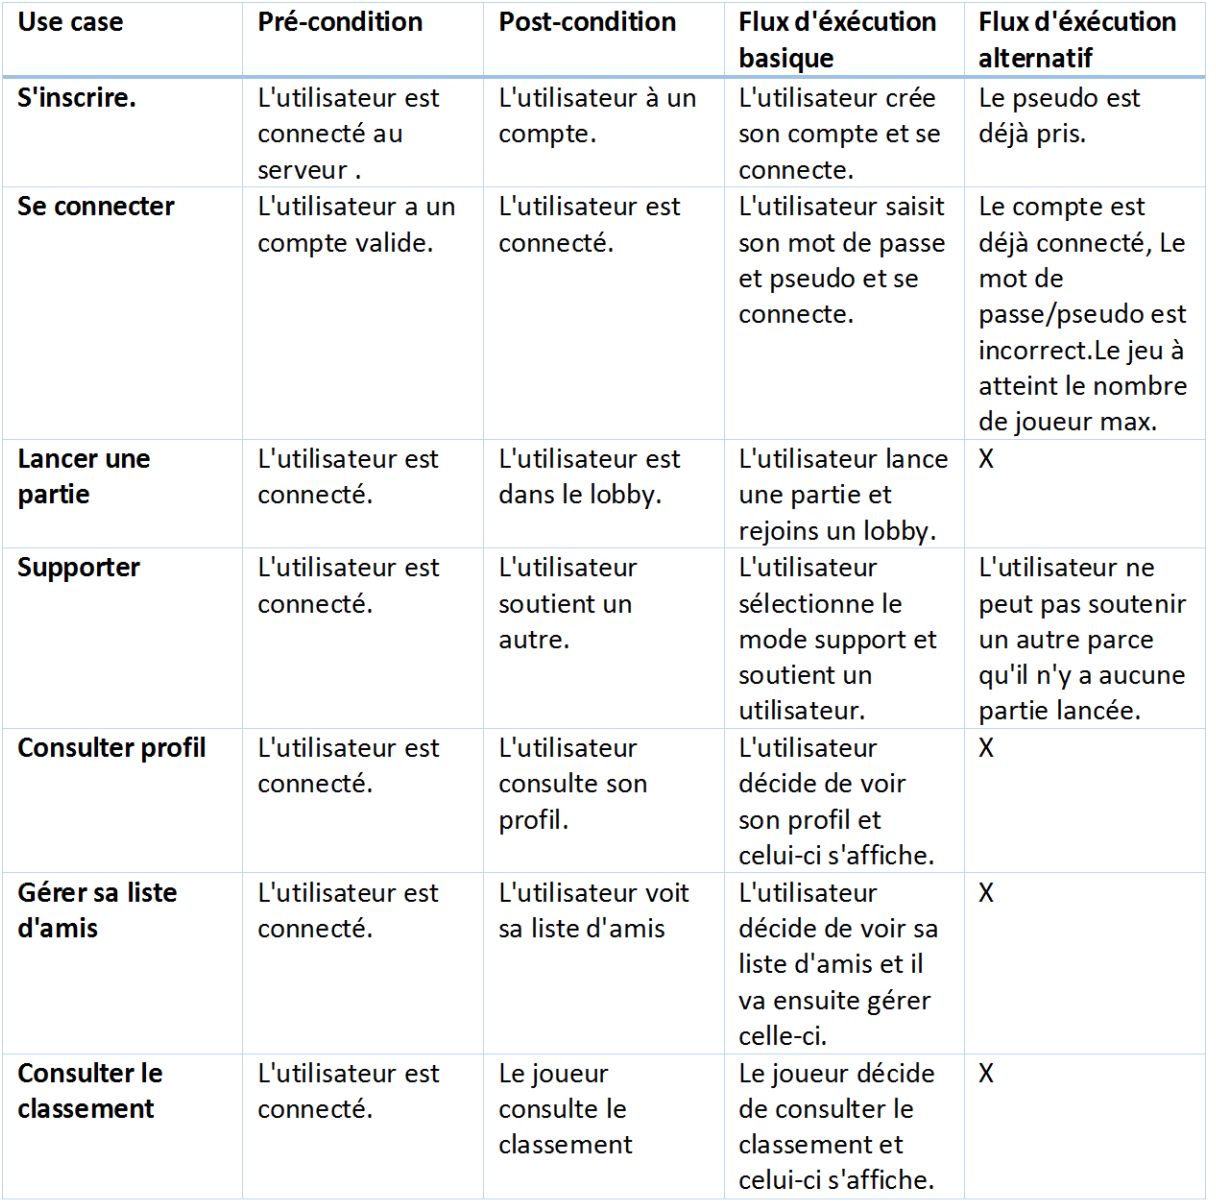
\includegraphics[height=12cm,width=16.45cm]{condition.png}
    \caption{Description diagramme use case avant une partie}   
  \label{fig:picture}
\end{center}
\end{figure}

\begin{figure}[H]
\begin{center}
    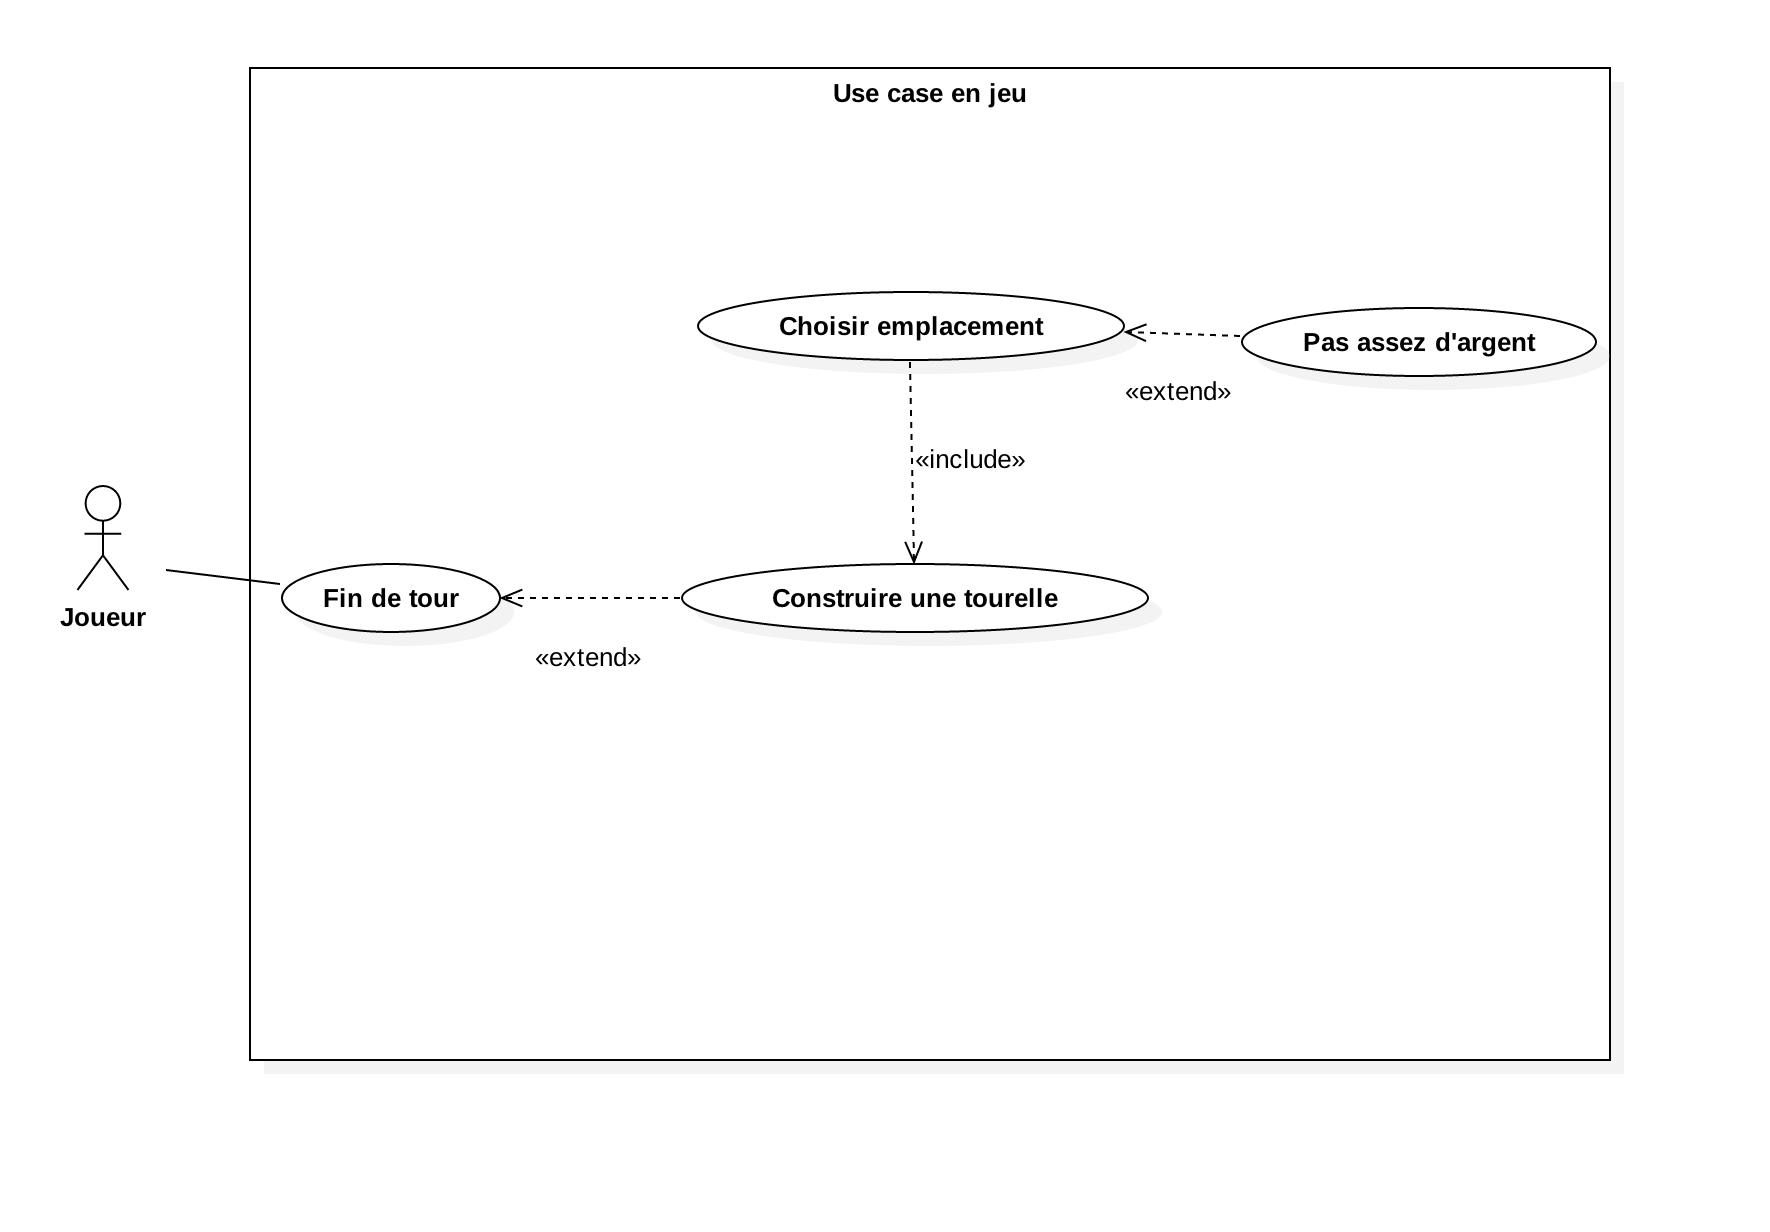
\includegraphics[height=13.5cm,width=17cm]{ingame_use_case.png}
     \caption{Diagramme uml en partie}   
  \label{fig:picture}
\end{center}
\end{figure}
%\newpage
\begin{figure}[H]
\begin{center}
    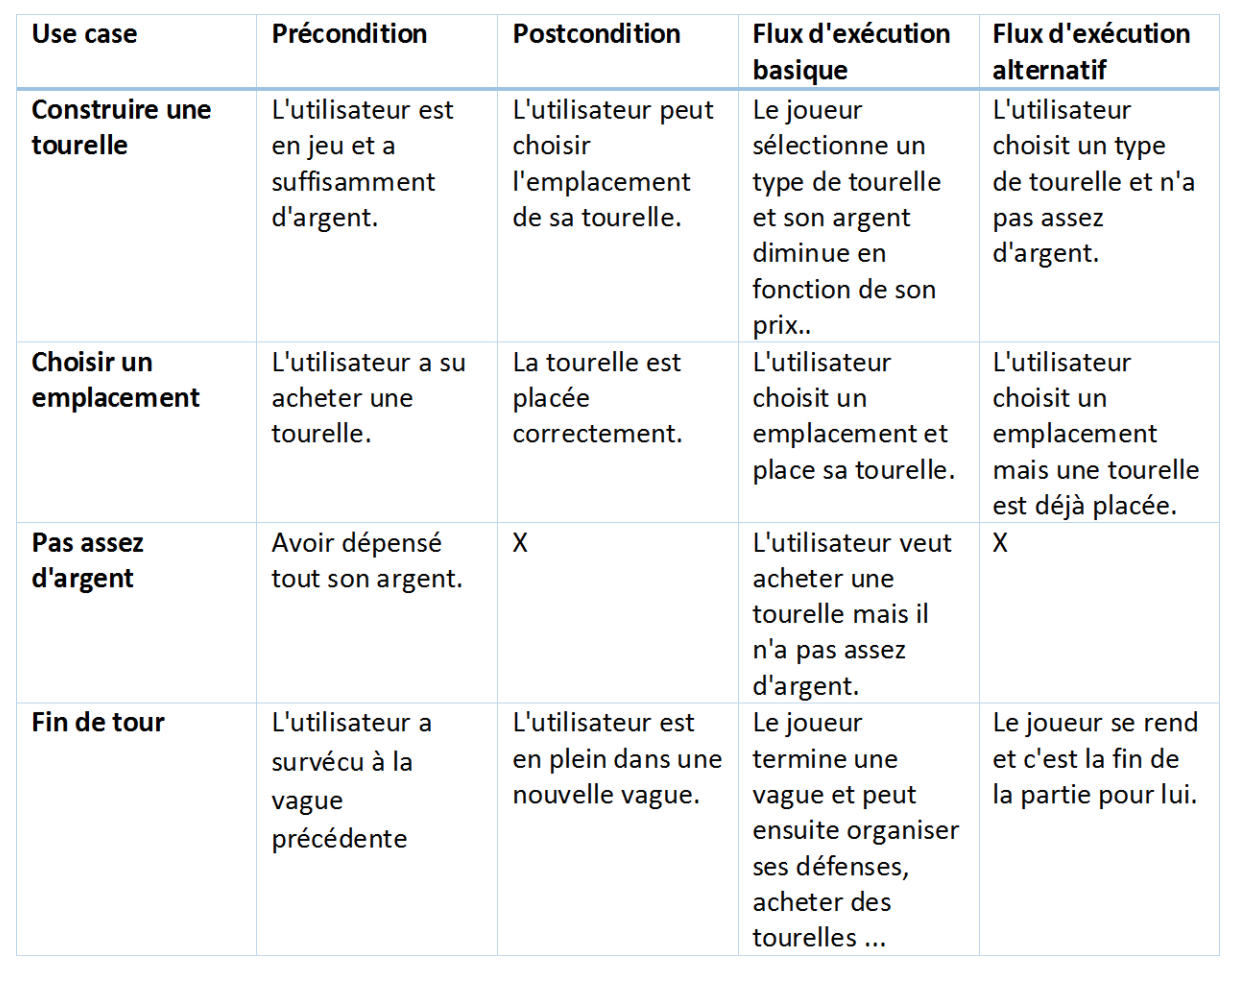
\includegraphics[height=13.5cm,width=17cm]{condition2.png}
     \caption{Diagramme uml en partie}   
  \label{fig:picture}
\end{center}
\end{figure}
%\begin{itemize}
%\item \textit{\textbf{Acteurs}} : ce use case a comme unique et principal acteur le \gls{joueur}\index{joueur}.\\

%\item \textit{\textbf{Pré-conditions}} : pour ce qui est des pré-conditions le \gls{joueur} doit être connecté et a dû lancer une partie\index{partie}.\\

%\item \textit{\textbf{Post-conditions}} : la seule post-condition est qu'une fois la partie\index{partie} terminée, le \gls{joueur} retourne au menu\index{menu}.\\

%\item \textit{\textbf{Flux d'exécution}} : pour ce qui est du déroulement basique, une fois en jeu le \gls{joueur}\index{joueur} peut construire des tourelles, consulter la description de celles-ci, il peut également les améliorer, les vendre, mais aussi modifier les paramètres du jeu. Il existe également un flux d'exécution alternatif. Au lieu de jouer, l'\gls{utilisateur}\index{utilisateur} peut être tout simplement un spectateur de la partie\index{partie}.

%\end{itemize}




\newpage    
\subsection{Exigences non fonctionnelles}
Dans le cadre de ce projet plusieurs exigences non fonctionnelles ont été relevés.Premièrement plusieurs deadlines ont été mises en place.La première le 19-12-2016,la seconde pour le dimanche 5 mars et la dernière pour le 31 mars 2017.
En ce qui concerne les langages de programmation imposés, il s'agit du C et du langage C++.De même, le projet doit être capable de fonctionner sur plusieurs plateformes telles que linux,window et mac os.Les autres besoins relevés concernent plus le jeu et sont ceux-ci:
\begin{itemize}
    \item \textit{\textbf{Menu\index{menu} et interface intuitifs}}:\\
    En effet, un menu ou un interface peu intuitif nuit très vite à la l'expérience de l'utilisateur.Il est donc impérative que celui-ci si retrouve très facilement.
    \item \textit{\textbf{Animations graphiques}}:\\
    De même, un jeu parfaitement bien animé, plaisant à regarder améliore l'expérience apporté par celui-ci.
    \item \textit{\textbf{Maniabilité}}:\\
    Outre le fait que fait que l'interface doit être intuitive, il est également important d'avoir un jeu ayant une bonne maniabilité.
    
\end{itemize}
    
\subsection{Exigence de domaine}

\begin{itemize}
	\item Le jeu doit être multijoueur, les différents \glspl{utilisateur}\index{utilisateur} connectés sur un même \gls{serveur}\index{serveur} doivent pouvoir agir sur le terrain.
   \item  L'abandon\index{abandon} d'un des \glspl{joueur}\index{joueur} ne doit pas empêcher les autres de terminer leur partie\index{partie}. 
   \item Un jeu de \gls{Tower Defense}\index{Tower Defense} est un jeu de 2 à 4 \glspl{joueur}\index{joueur} qui ont chacun une partie\index{partie} de la carte.
   \item Chacun des \glspl{joueur}\index{joueur} a sa base\index{base} dans chaque coin du jeu.
   \item Les \glspl{ennemi}\index{ennemi} apparaissent au milieu de la carte, leur vagues sont identiques pour chaque \gls{joueur}.
   \item La partie\index{partie} se déroule sous forme de vagues successives d’\glspl{ennemi}\index{ennemi} jusqu’à ce que la partie\index{partie} se termine.
   \item  Les \glspl{joueur}\index{joueur} peuvent améliorer ou acheter des tours à tout moment de la partie\index{partie}.
   \item  La partie se termine si le temps est écoulé dans le cas d’une partie\index{partie} en mode chrono\index{mode chrono} ou s’il ne reste que un \gls{joueur} vivant dans le cas d’une partie classique\index{partie classique}.
\end{itemize}
\newpage
\section{Besoin du système}
\subsection{Exigences fonctionnelles}
Les exigences fonctionnelles du système sont les besoins expliqué par le client \index{client} mais qui n'ont aucun lien avec celui-ci. Elles sont donc implicite et après analyses des exigences nous avons pu discerner plusieurs exigences fonctionnelles: \\

\begin{itemize}
    \item \textit{\textbf{Démarrer\&Initier une partie\index{partie}}}:\
    Fonction qui initie une partie \index{partie} lorsqu'un \gls{utilisateur}\index{utilisateur} en fait la demande. Pour cela différentes données sont nécessaires tels que le mode de jeu et le nombre de \glspl{joueur}\index{joueur} requis pour la partie\index{partie}. Une fois le nombre de joueur atteint pour une partie\index{partie}, le serveur lance automatiquement la partie chez tout les \glspl{utilisateur} et rafraîchit leur interface.
    \item \textit{\textbf{Trouver une partie \index{partie}}}:\\ Lorsqu'un \gls{utilisateur} veut jouer une partie ou en rejoindre une pour être le soutient d'un autre \gls{utilisateur}, le serveur fait appel au matchmaking qui permet de regrouper plusieurs personnes dans un même \index{salon} de jeu, en attendant le début d'une partie.La partie commençant quand le \index{salon} est plein.
    \item \textit{\textbf{Partie}}:\\
    Cela est une composante importante du programme. La partie \index{partie} se compose de divers fonctionnalités: placer une tours, vérification de victoire, défaite et établissement des scores et récompenses attribués à chaque à \gls{joueur}.
    \item \textit{\textbf{Classement}}:\\
    Regroupe tout les scores des joueurs classé du meilleur au moins bon score et est mis à jours après chaque partie.
\end{itemize}

\subsection{Exigences non fonctionnelles}
Les exigences non fonctionnelles sont très importantes pour réaliser correctement le projet.Cette section reprend donc un certain nombre d'aspect qui n'ont pas été déclaré clairement par le client.
Par ailleurs, il est évident que un certains nombre d’interactions entre le \gls{client}\index{client} et le \gls{serveur}\index{serveur} seront mises en place, vu que le projet est un programme devant être jouable en réseau.\\Voici quelques unes de ces interactions:


\begin{itemize}
    \item Création d'un \gls{compte}\index{compte} \gls{utilisateur}\index{utilisateur} et connexion de celui-ci au système.
    \item Mise à jour des amis d'un joueur. 
    \item Organisation.
    \item Réactivité.
\end{itemize}

De plus, les différents points qui sont repris ci dessus ne reflètent que les aspects clés qui ont été déterminé suite à la rencontre avec le client.\\
%\newpage
\subsection{Design et fonctionnement du système}
Cette sections reprends les diagrammes permettant de décrire l'architecture du système et son fonctionnement. Les différents diagrammes UML ayant été utilisé sont diagrammes de classe, de séquence et d'activité. Veuillez consulter la section uml pour voir ses diagrammes en entier.
\begin{figure}[H]
  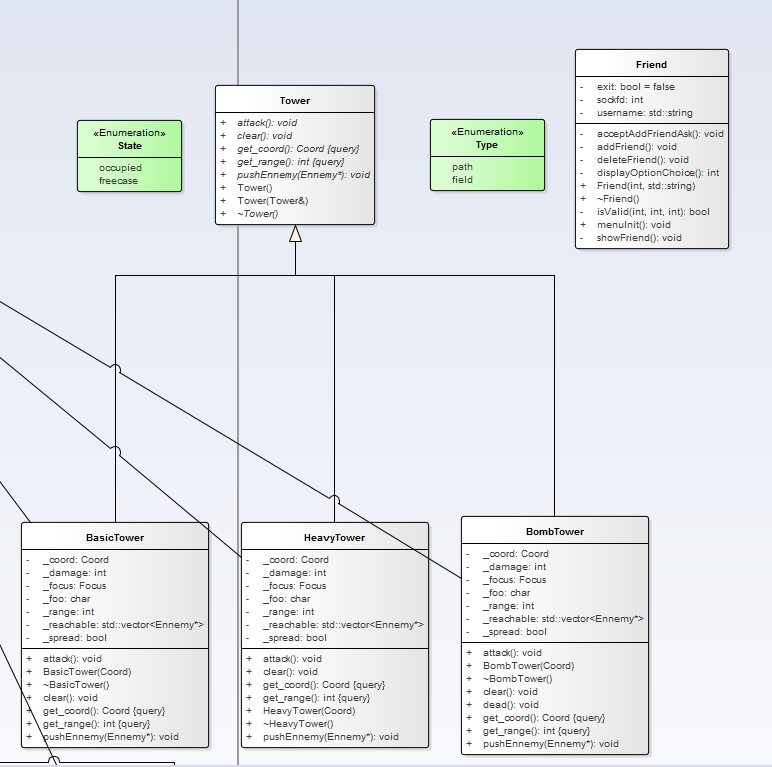
\includegraphics[height=20cm,width=20cm]{classDiagram1.png}
  \caption{Diagramme de classe partie terminale}
   \label{fig:picture}
 \end{figure}

  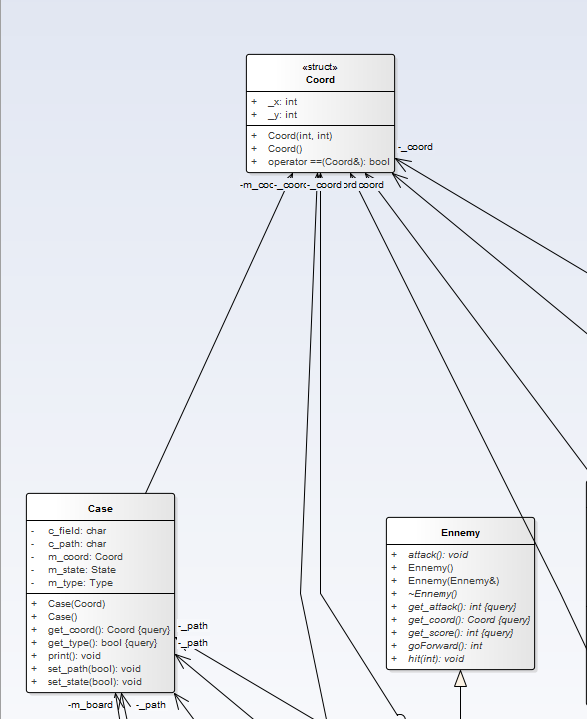
\includegraphics[height=20cm,width=15cm]{classDiagram2.png}

  


  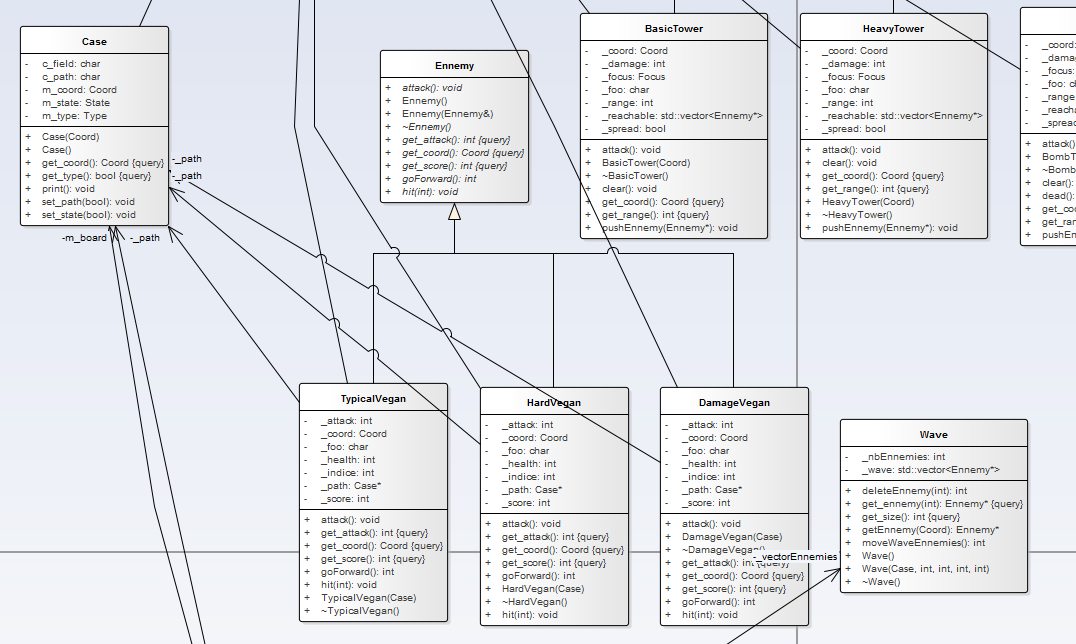
\includegraphics[height=20cm,width=20cm]{classDiagram3.png}

  

  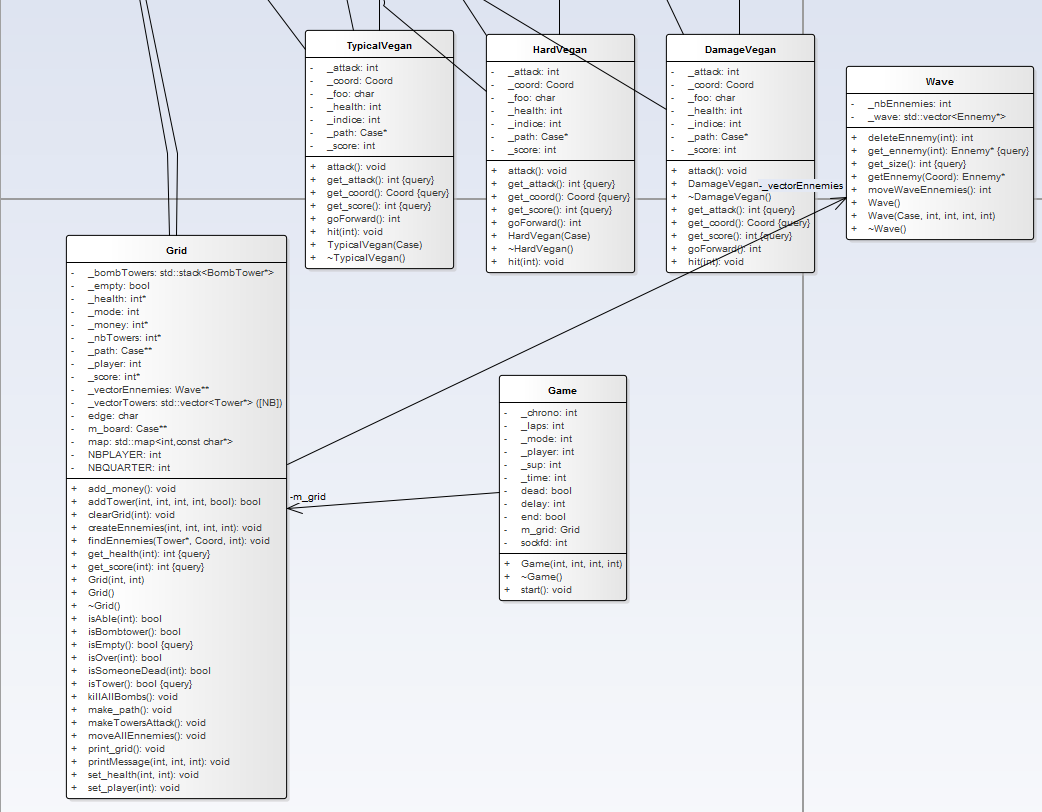
\includegraphics[height=20cm,width=20cm]{classDiagram4.PNG}


  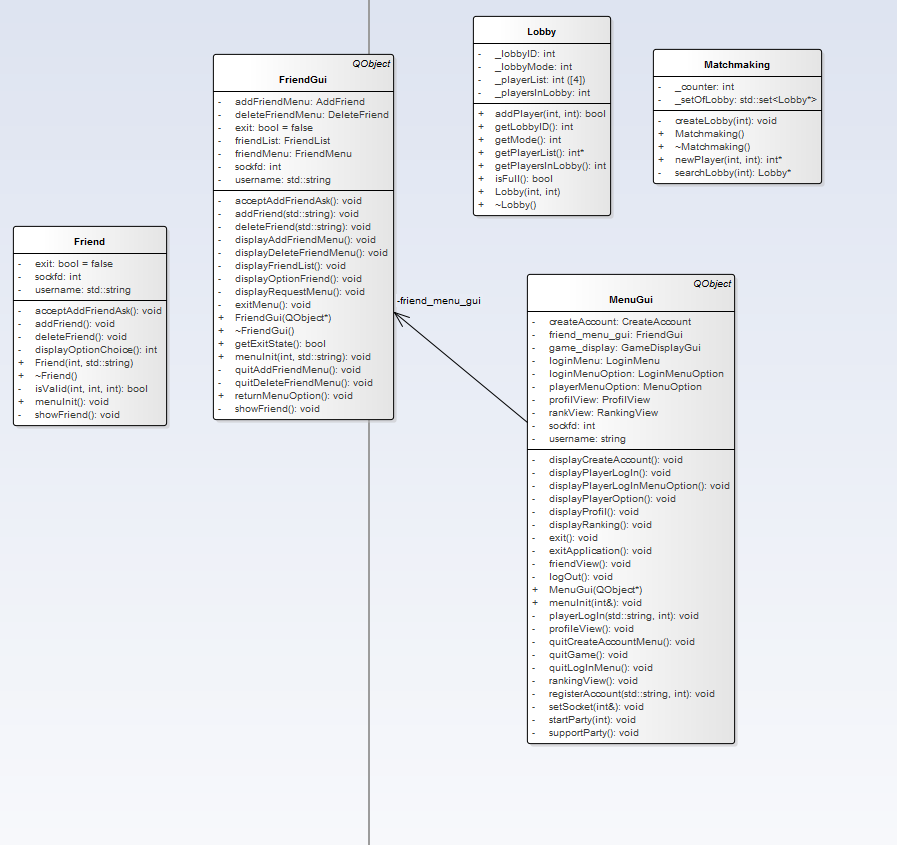
\includegraphics[height=20cm,width=20cm]{classDiagram5.png}


\newpage
\begin{figure}[H]
  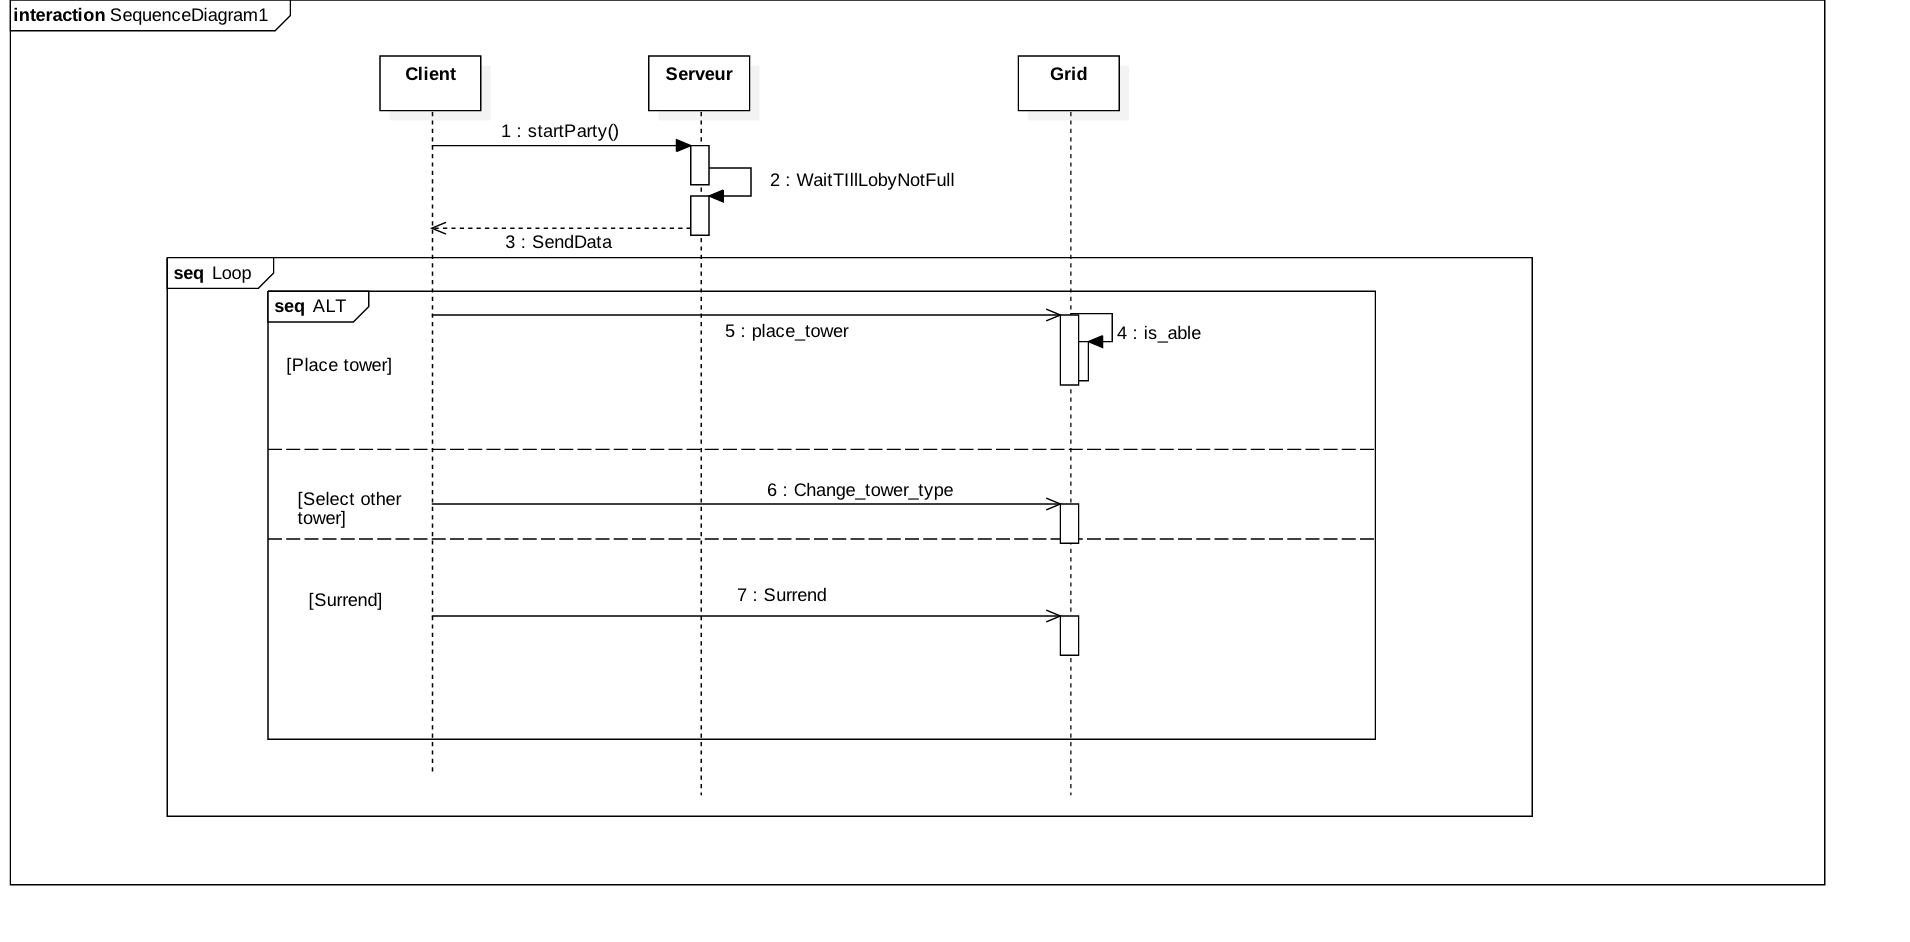
\includegraphics[height=13cm,width=19cm]{SequenceINGAME.png} 
  \caption{Diagramme de sequence en jeu}
   \label{fig:picture}
 \end{figure}


\newpage
\section{Modules}
Pour faciliter le développement du projet mais aussi pour avoir une certaine cohérence, le programme a été découpé en plusieurs modules.Ceux-ci sont détaillés ci-dessous.
\section{Module Match}
Cette section explique la façon dont le jeu est joué et la manière dont on a implémenté le gameplay.
\subsection{Gameplay}
Entre chaque vague l'utilisateur \index{utilisateur} à la possibilité de:
\begin{itemize}
    \item[$\bullet$] Placer une tourelle.
    \item[$\bullet$] Surrend (abandonner la partie).
\end{itemize}
Parmi les tourelles disponibles l'utilisateur \index{utilisateur} peut placer 3 types de tourelles:
\begin{itemize}
    \item[$\bullet$] Basique coûtant 100 "Money".
    \item[$\bullet$] Heavy tourelle plus chère mais plus puissante et coûtant 200 "Money".
    \item[$\bullet$] Bomb tourelle qui dure qu'une seule vague mais dévastatrice avec un prix de 300 "Money".
\end{itemize}
Bien évidemment le joueur peut placer autant de tourelle qu'il veut, tant que celui-ci a assez de "Money" et dans les limites du temps entre chaque vagues.
\bigskip
\par
Le terrain est séparé en 4 parties pour 4 joueurs et chacune de ces parties comportent un couloir par lequel des vagues de monstres apparaissent.
Les monstres sont représentés par différents symboles et clignotent en rouge lorsqu'ils se font toucher par une tourelle.
\subsection{Choix d'implémentation}
Cette partie décrit des choix personnels quant au gameplay et donc non explicités par le client. Ceux-ci sont repris ci-dessous.
\begin{itemize}
\item[$\bullet$] Tourelle : celles-ci regardent à chaque moment si des ennemis se trouvent à leur porté et si le choix de la cible se porte vers l'ennemi le plus proche de la base.
\item[$\bullet$] Ennemis : lorsqu'un ennemi est en mouvement celui-ci vérifie sa vie. Si elle est à zéro suite à l'attaque d'une tourelle, ils disparaissent, sinon ils continuent d'avancer jusque la base.
\end{itemize}
\newpage
\subsection{Support}
Outre le fait qu'un support est un utilisateur comme un autre, celui-ci ne joue pas vraiment une partie et rejoins quand une partie est déjà lancée. De manière générale, le support indique le pseudo de l'utilisateur qu'il souhaite soutenir et est placé dans une queue. Suite à ça, si l'utilisateur que le support souhaite soutenir est en jeu, L'utilisateur étant supporté gagnera automatiquement 100 de "Money".Finalement, le support devra attendre la fin de la partie et ne pourra donc plus rien faire.
\section{Communication}
\subsection{Architecture générale}
\subsubsection{Mode de fonctionnement}
L'idée générale pour gérer cette communication entre le client et le serveur est la mise en place de nombreux recv et send. De cette manière la communication entre les deux suit une certaine logique. Cette façon de communiquer peut paraître dangereuse à cause d'un recv bloquant mais il n'en est rien. Un soin particulier à été apporté à l'emplacement des envoies et des recv, de sorte à ce que la communication entre le client et le serveur soit la plus fluide possible.
\subsubsection{Architecture du client}
De la même manière, le \index{client} client fait appel à différents objets qui vont directement communiquer avec le serveur via des send et des recv. Le tout étant encore une fois agencé avec précaution et une certaine logique, de manière à ce que la communication client-serveur se fasse le plus facilement possible.
\subsubsection{Architecture du serveur}
Le serveur va dédié un \gls{thread} \index{thread} à chaque fois qu'un nouveau \gls{utilisateur}\index{utilisateur} va faire une nouvelle demande de connexion.De cette manière, le serveur garantis la même interaction quel que soit l' \gls{utilisateur}\index{utilisateur}. De même, le serveur est celui-ci qui se charge de toute les requêtes envoyés par le client.Celui-ci se charge donc de l'écriture et lecture dans un fichier.
\subsection{Communication inter-\gls{thread}\index{thread}}
Une communication entre \gls{thread} \index{thread} est nécessaire lorsque tous les utilisateurs \index{utilisateurs} sont en jeu. En fonction de l'action de l'utilisateur \index{utilisateur} le serveur va recevoir plusieurs informations.
\begin{itemize}
\item[$\bullet$] Placement d'une tourelle: coordonnées en x et y, l'id de l'utilisateur. \index{utilisateur} et le type de la tourelle.
\item[$\bullet$] Surrender: des coordonnées et l'id de l'utilisateur \index{utilisateur}.
\end{itemize}
Une fois les informations obtenues, le serveur va automatiquement envoyer les données à tous les autres utilisateurs. Par conséquent, tous les utilisateurs voient ce que les autres utilisateurs font à tout moment de la partie.
\newpage
\section{Module stockage des données}
\subsection{Stockage des comptes}
Pour sauvegarder toutes les données telles que :
\begin{itemize}
\item[$\bullet$] le \gls{pseudo} \index{pseudo}
\item[$\bullet$] le mot de passe
\item[$\bullet$] une valeur indiçant l'état de l'utilisateur(connecté ou non) \index{utilisateur}
\end{itemize}
nous avons donc créé un fichier texte appelé "account.txt" qui gardera donc à tout moment ces données. Le but premier du projet n'étant pas la sécurité mais bien un jeu fonctionnel, nous avons décidé de mettre en place un système de fichier texte et non une base de données car nous sommes plus familiarisé avec un système de fichiers. Bien évidemment si le fichier n'existe pas, il sera créé par le serveur.
\subsection{Stockage de la liste d'amis}
De même, pour chaque \index{utilisateur} \gls{utilisateur} un fichier texte sous son nom est crée pour contenir sa liste d'amis. Une demande d'ami est représenté dans le fichier par une valeur "0" à côté du pseudo \index{pseudo} de l'utilisateur ayant envoyé la demande. Ce fichier sous la forme "NomUtilisateur.txt" va servir pour de nombreuses opérations telle que :
\begin{itemize}
    \item[$\bullet$] La visualisation du profil.
    \item[$\bullet$] La consultation de la liste d'amis.
    \item[$\bullet$] accepter un amis.
    \item[$\bullet$] ajouter un amis.
    \item[$\bullet$] supprimer un amis.
\end{itemize}
 Une valeur "1" signifie que les deux utilisateurs\index{utilisateurs} sont déjà amis.
 \subsection{stockage de la vague d'ennemis}
Tout comme pour les comptes et la liste d'amis, nous avons décider de continuer sur un système de fichier, et nous avons donc créer un fichier pour stocker les vagues d'ennemis. Plus précisément, celui-ci est composé de 4 champs qui indiquent:
\begin{enumerate}
    \item Le nombre total d'ennemis par vague.
    \item le nombre total d'ennemis de type "a".
    \item le nombre total d'ennemis de type "b".
    \item le nombre total d'ennemis de type "c". 
\end{enumerate}


\subsection{Accès au données}
Finalement, le client ne contient donc aucune données. À chaque requêtes telles qu'une demande d'ami, consulter son profil... Celui-ci doit passer par le serveur pour recevoir une réponse. Cette façon de faire bien que coûteuse en performance(lecture dans les fichiers, transfert d'informations entre le client\index{client} et le serveur \index{serveur}...) garantit une séparation entre le tâche du \index{client} client et du serveur \index{serveur}. Si\index{utilisateur} l'utilisateur demande de se connecter, la vérification passera donc par le serveur.
\begin{figure}[H]
  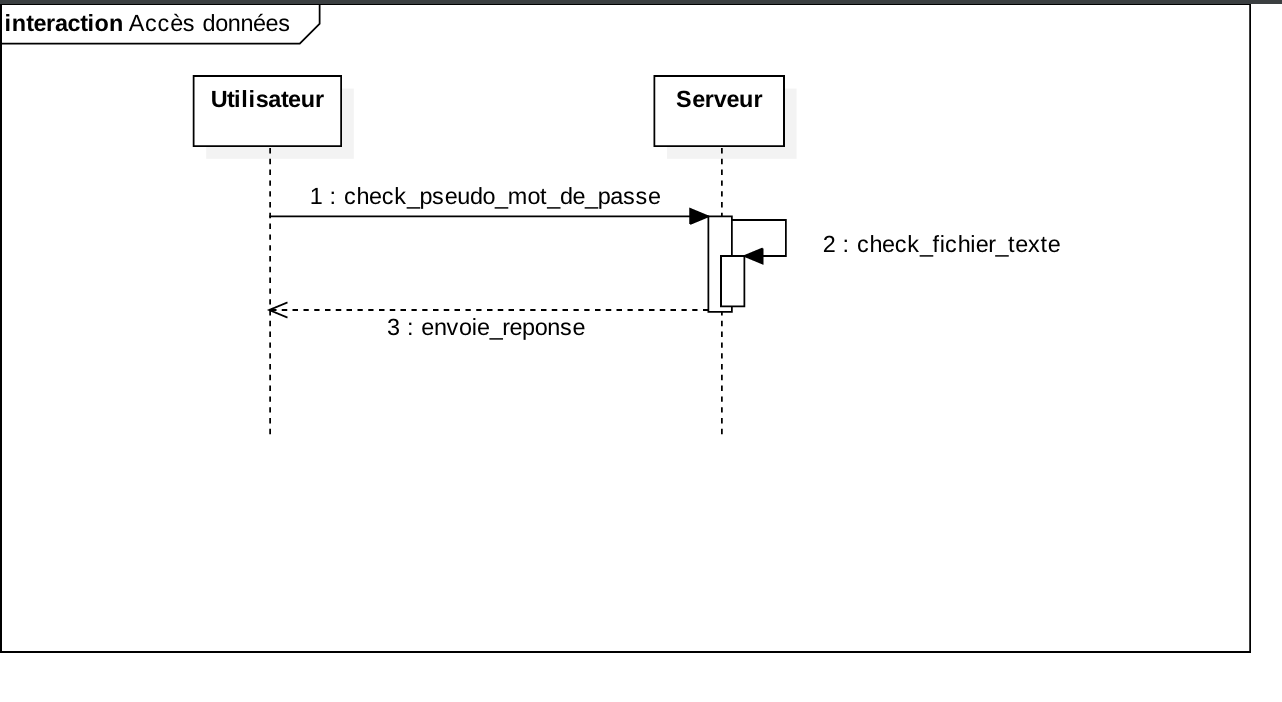
\includegraphics[height=13cm,width=19cm]{RequestSequence.png} 
    \caption{Diagramme de sequence du Matchmaking.}
   \label{fig:picture}
 \end{figure}
\newpage 
\section{Matchmaking}
Lorsqu'un utilisateur \index{utilisateur} veut jouer celui-ci va être repris par la classe Matchmaking. Ainsi, le matchmaking se chargera de placer chaque utilisateurs \index{utilisateurs} dans le bon lobby, en fonction du mode de jeu choisit par celui-ci, si le lobby est plein, le matchmaking va automatiquement créer un nouveau salon. Un lobby est considéré comme plein lorsque la limite max pour ce lobby est atteinte. Il est limité à 4 utilisateurs pour le mode par équipe et le mode versus, pour ce qui est du mode chrono, un seul utilisateur suffit. 
 \begin{figure}[H]
  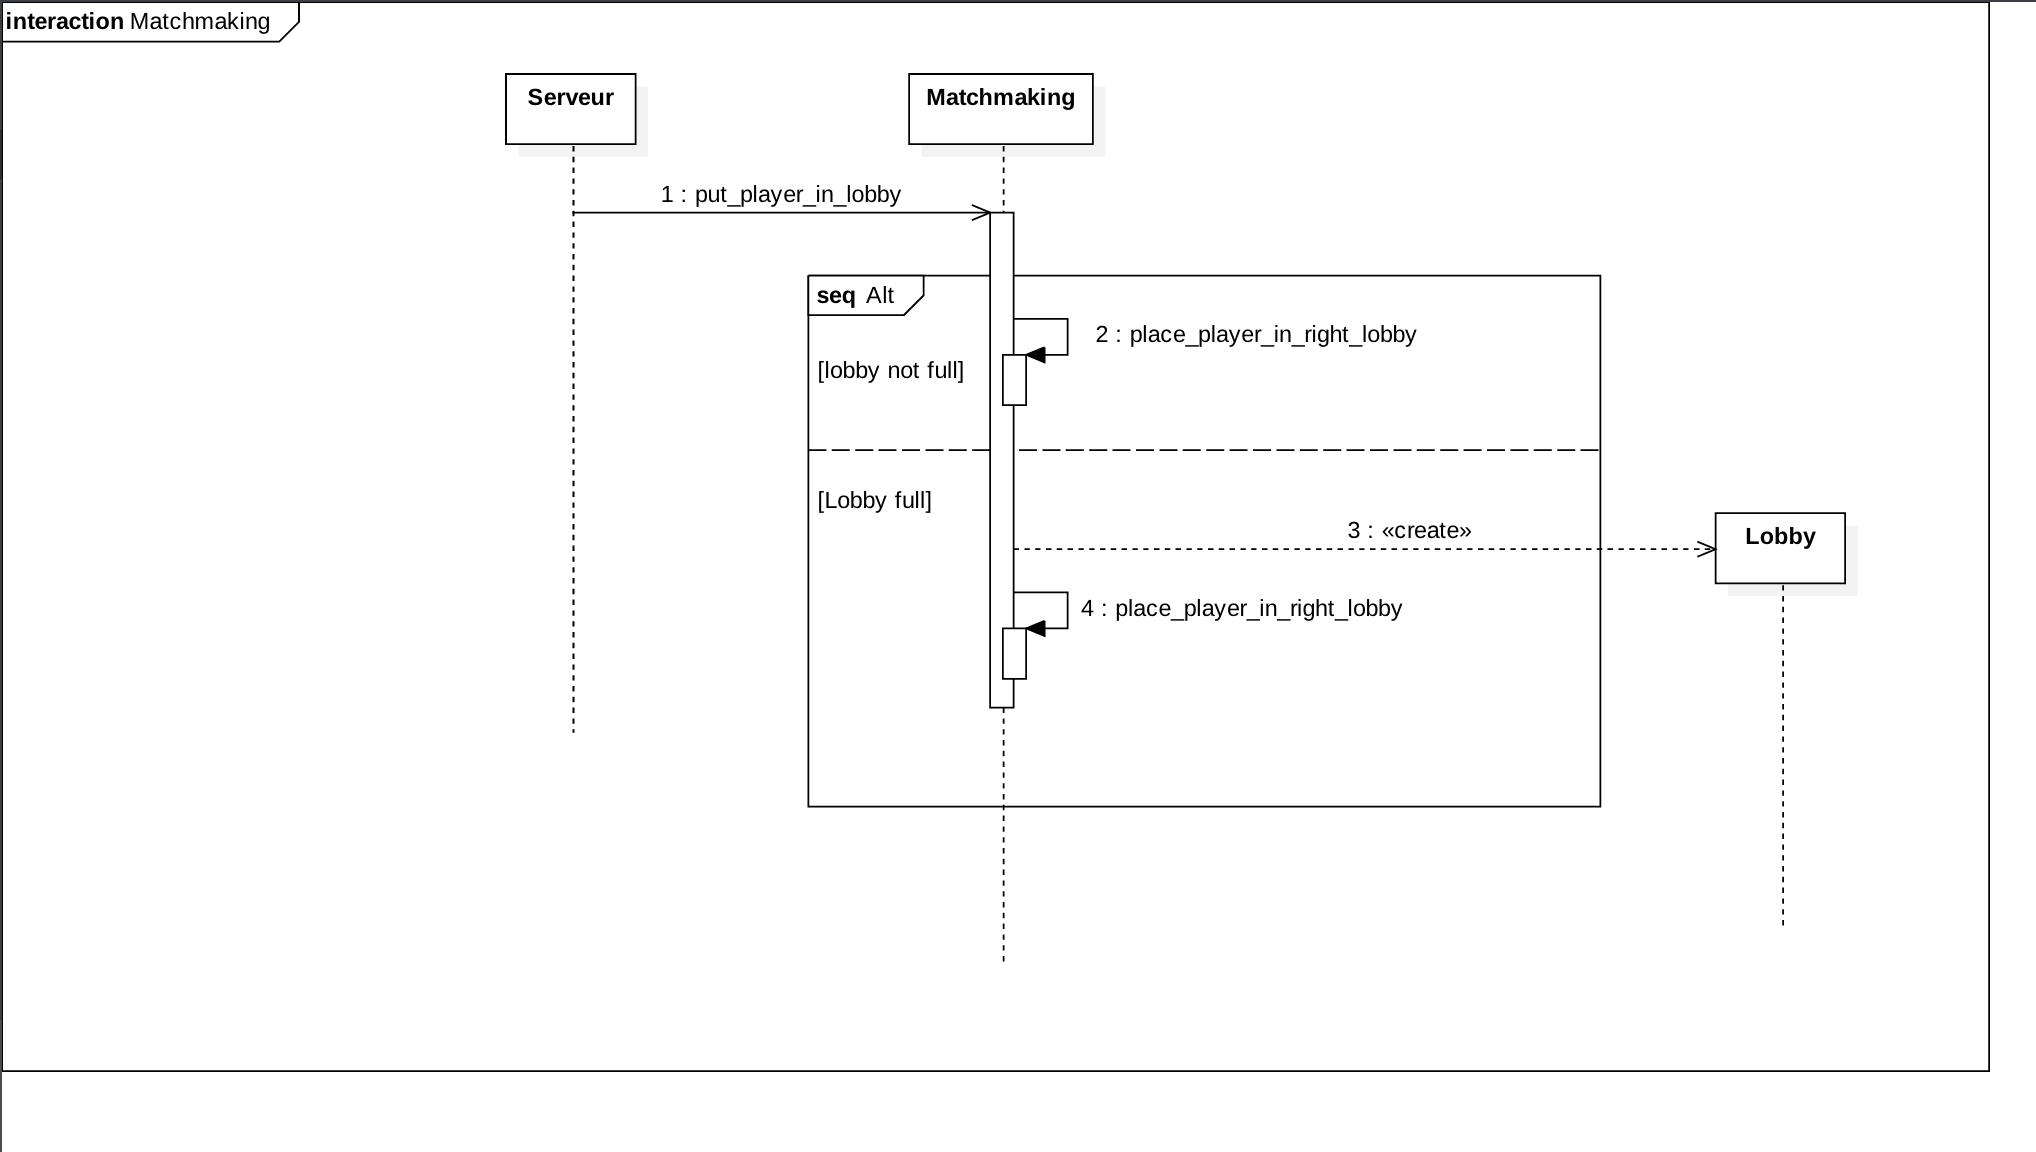
\includegraphics[height=13cm,width=19cm]{MatchSequence.png} 
    \caption{Diagramme de sequence du Matchmaking.}
   \label{fig:picture}
 \end{figure}
\newpage
\section{Affichage console}
La gestion de l'affichage a été faîte de manière à représenter à tout moment les actions que le client décide de faire. De ce fait, on peut donc séparer l'affichage en 3 grosses parties.
\begin{itemize}
\item[]Inscription/connexion
\item[]le menu représentant les choix possibles(consulter la liste d'amis...)
\item[]L'affichage du jeu.
\end{itemize}
\subsection{Inscription / connexion}
La première partie consiste donc à l'inscription ou la connexion d'un \index{utilisateur} utilisateur.Ainsi, L'utilisateur est invité à saisir un pseudo \index{pseudo} et un mot de passe dans le cas où il veut se connecter, et de manière similaire il est convié à saisir un nouveau pseudo et un nouveau mot de passe dans le cas où celui-ci veut s'inscrire.
\begin{center}
    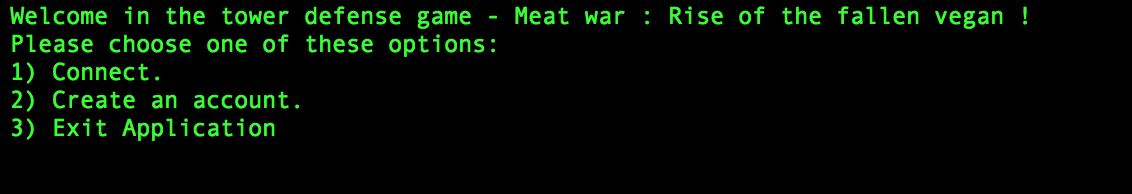
\includegraphics[height=5cm,width=14cm]{login.png}
\end{center}
\newpage
\subsection{Menu}
Cette partie est donc accessible après que l'utilisateur\index{utilisateur} s'est connecté, suite à une confirmation de la validité du compte réalisé par le serveur\index{serveur}.Ensuite, 6 options sont mises à disposition du joueur;
\begin{itemize}
\item[$\bullet$] Lancer une partie.
\item[$\bullet$] Soutenir un joueur dans une partie.
\item[$\bullet$] Visualisation du profil.
\item[$\bullet$] Affichage du classement.
\item[$\bullet$] Accéder au gestionnaire d'amis.
\item[$\bullet$] Quitter.
\end{itemize}
\begin{center}
    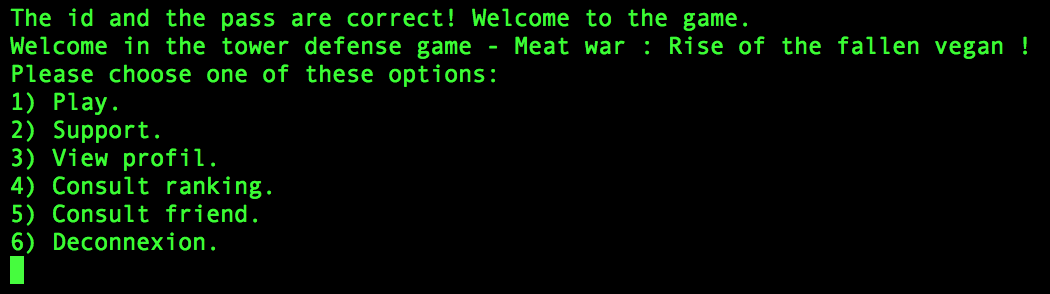
\includegraphics[height=5cm,width=14cm]{menu.png}
\end{center}
  
De manière similaire l'accès au gestionnaire d'ami mène à plusieurs nouveaux choix:
\begin{itemize}
\item[$\bullet$] Ajout d'un ami.
\item[$\bullet$] Suppression d'un ami.
\item[$\bullet$] Accepter une demande d'ami.
\item[$\bullet$] Consulter sa liste d'ami.
\item[$\bullet$] Quitter.
\end{itemize}
L'ensemble des ces méthodes sont donc disponible dans la classe Menu et dans la classe Friend.
\newpage
\subsection{Affichage du jeu}
L'affichage en jeu est réparti par plusieurs objets. De manière générale, c'est la classe \textit{\textbf{grid}} qui se charge de l'affichage de la carte mais aussi des différentes informations telles que:
\begin{itemize}
\item[$\bullet$] La vie des différents utilisateurs. \index{utilisateur}
\item[$\bullet$] Le score des utilisateurs. \index{utilisateur}
\item[$\bullet$] L'argent des utilisateurs.\index{utilisateur}
\end{itemize}
D'autres part l'affichage des différents monstres(Végan) est délégué à la classe \textit{\textbf{Ennemy}}. Finalement, il ne reste plus que l'affichage des tourelles \index{tourelle} est c'est la classe \textit{\textbf{Tower}} qui s'en charge.
%Demander à maiki.

\newpage
\section{Interface graphique}
L'interface graphique a été réalisé en dernier lieu, se joignant ainsi au jeu déjà préconçu. Pour ce faire nous avons décidé de laisser le choix à \index{utilisateur}l'utilisateur, celui-ci peut donc choisir entre l'interface graphique et l'ancienne partie sur terminal. Sur les différentes bibliothèques disponibles, nous avons choisit "qt". De ce fait, plusieurs moyens ont été mis en place pour coller le plus possible au thème(Meat VS Vegan). Premièrement plusieurs fond d'écran sont disponible et appliqué dans le jeu. Ensuite, La carte en jeu à été totalement revu et transformé en une carte plus adapté au thème. Puis les options disponibles dans le terminal ont été retravaillées pour qu’elles soient évidemment plus visuelles et plus faciles d’utilisation.

\bigskip
\par
Pour l'implémentions de cette partie graphique nous avons dérivés des classes existantes de la bibliothèque "qt". De cette dérivation, nous avons donc apporté nos propres modifications personnalisées. De cette manière, nous avons une bonne structure orientée-objet et il suffit d'instancier l'objet là ou il le faut. Pour finir nous avons décidé de cacher les fenêtres au lieu de les détruire à chaque fois.

\begin{figure}[H]
  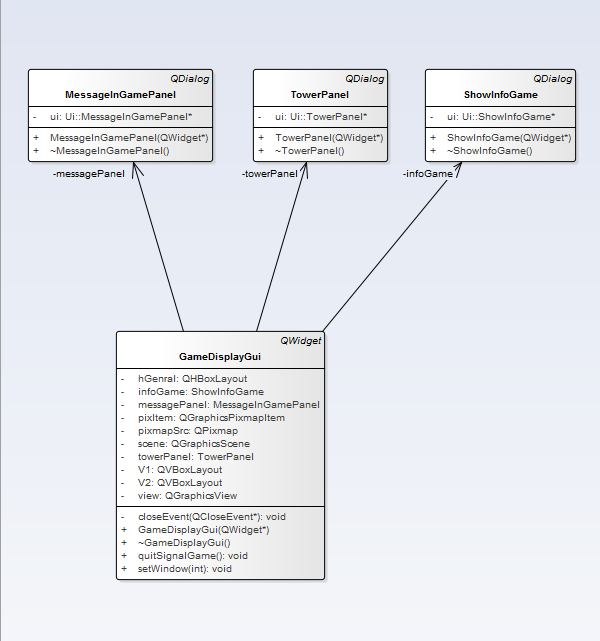
\includegraphics[height=20cm,width=20cm]{guiClass1.png}
  \caption{Diagramme de classe partie GUI}
   \label{fig:picture}
 \end{figure}

  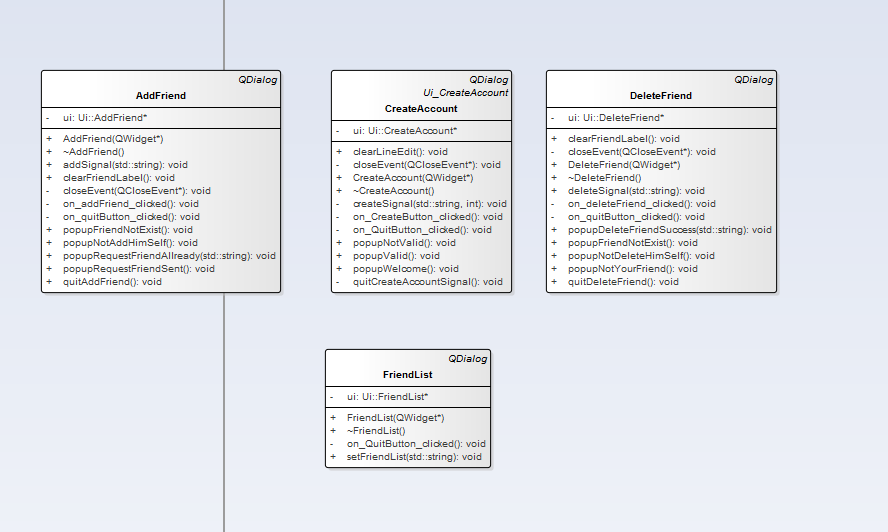
\includegraphics[height=20cm,width=20cm]{guiClass2.PNG}
  
 
  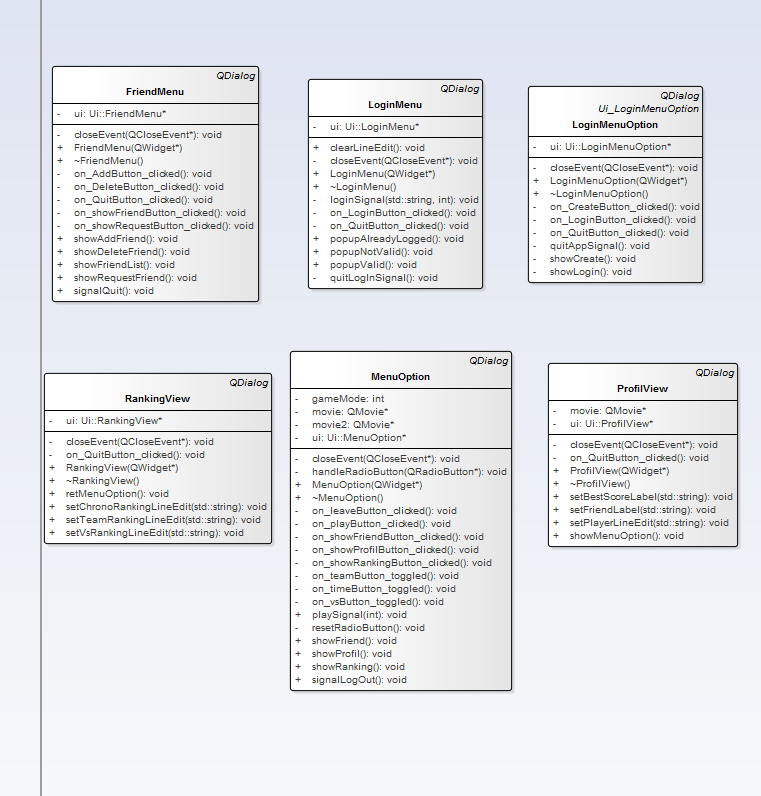
\includegraphics[height=20cm,width=20cm]{guiClass3.png}
  
\appendix 
\begin{center}
\begin{figure}[H]
    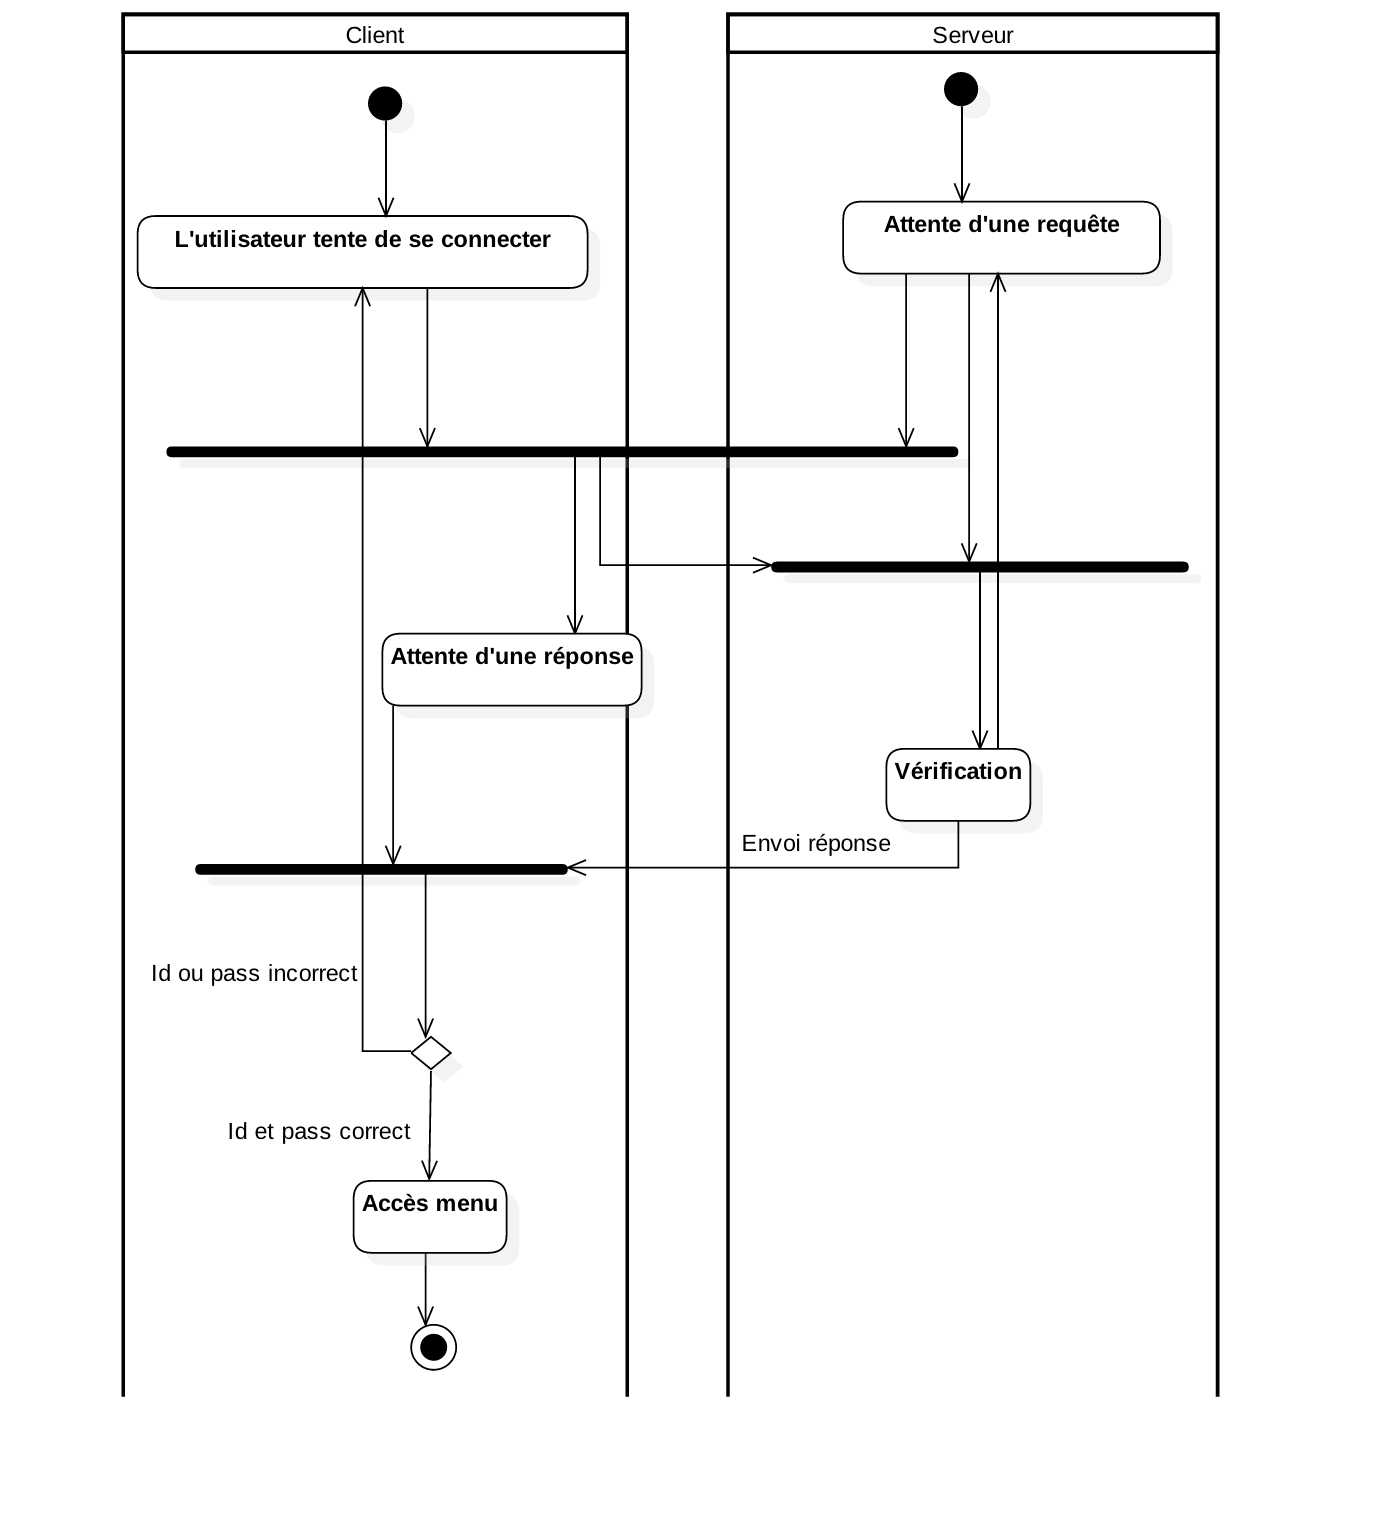
\includegraphics[height=18cm,width=18cm]{loginActi.png}
    \caption{Diagramme d'activité se connecter}
    \label{fig:picture}
 \end{figure}
\end{center}
\begin{center}
\begin{figure}[H]
    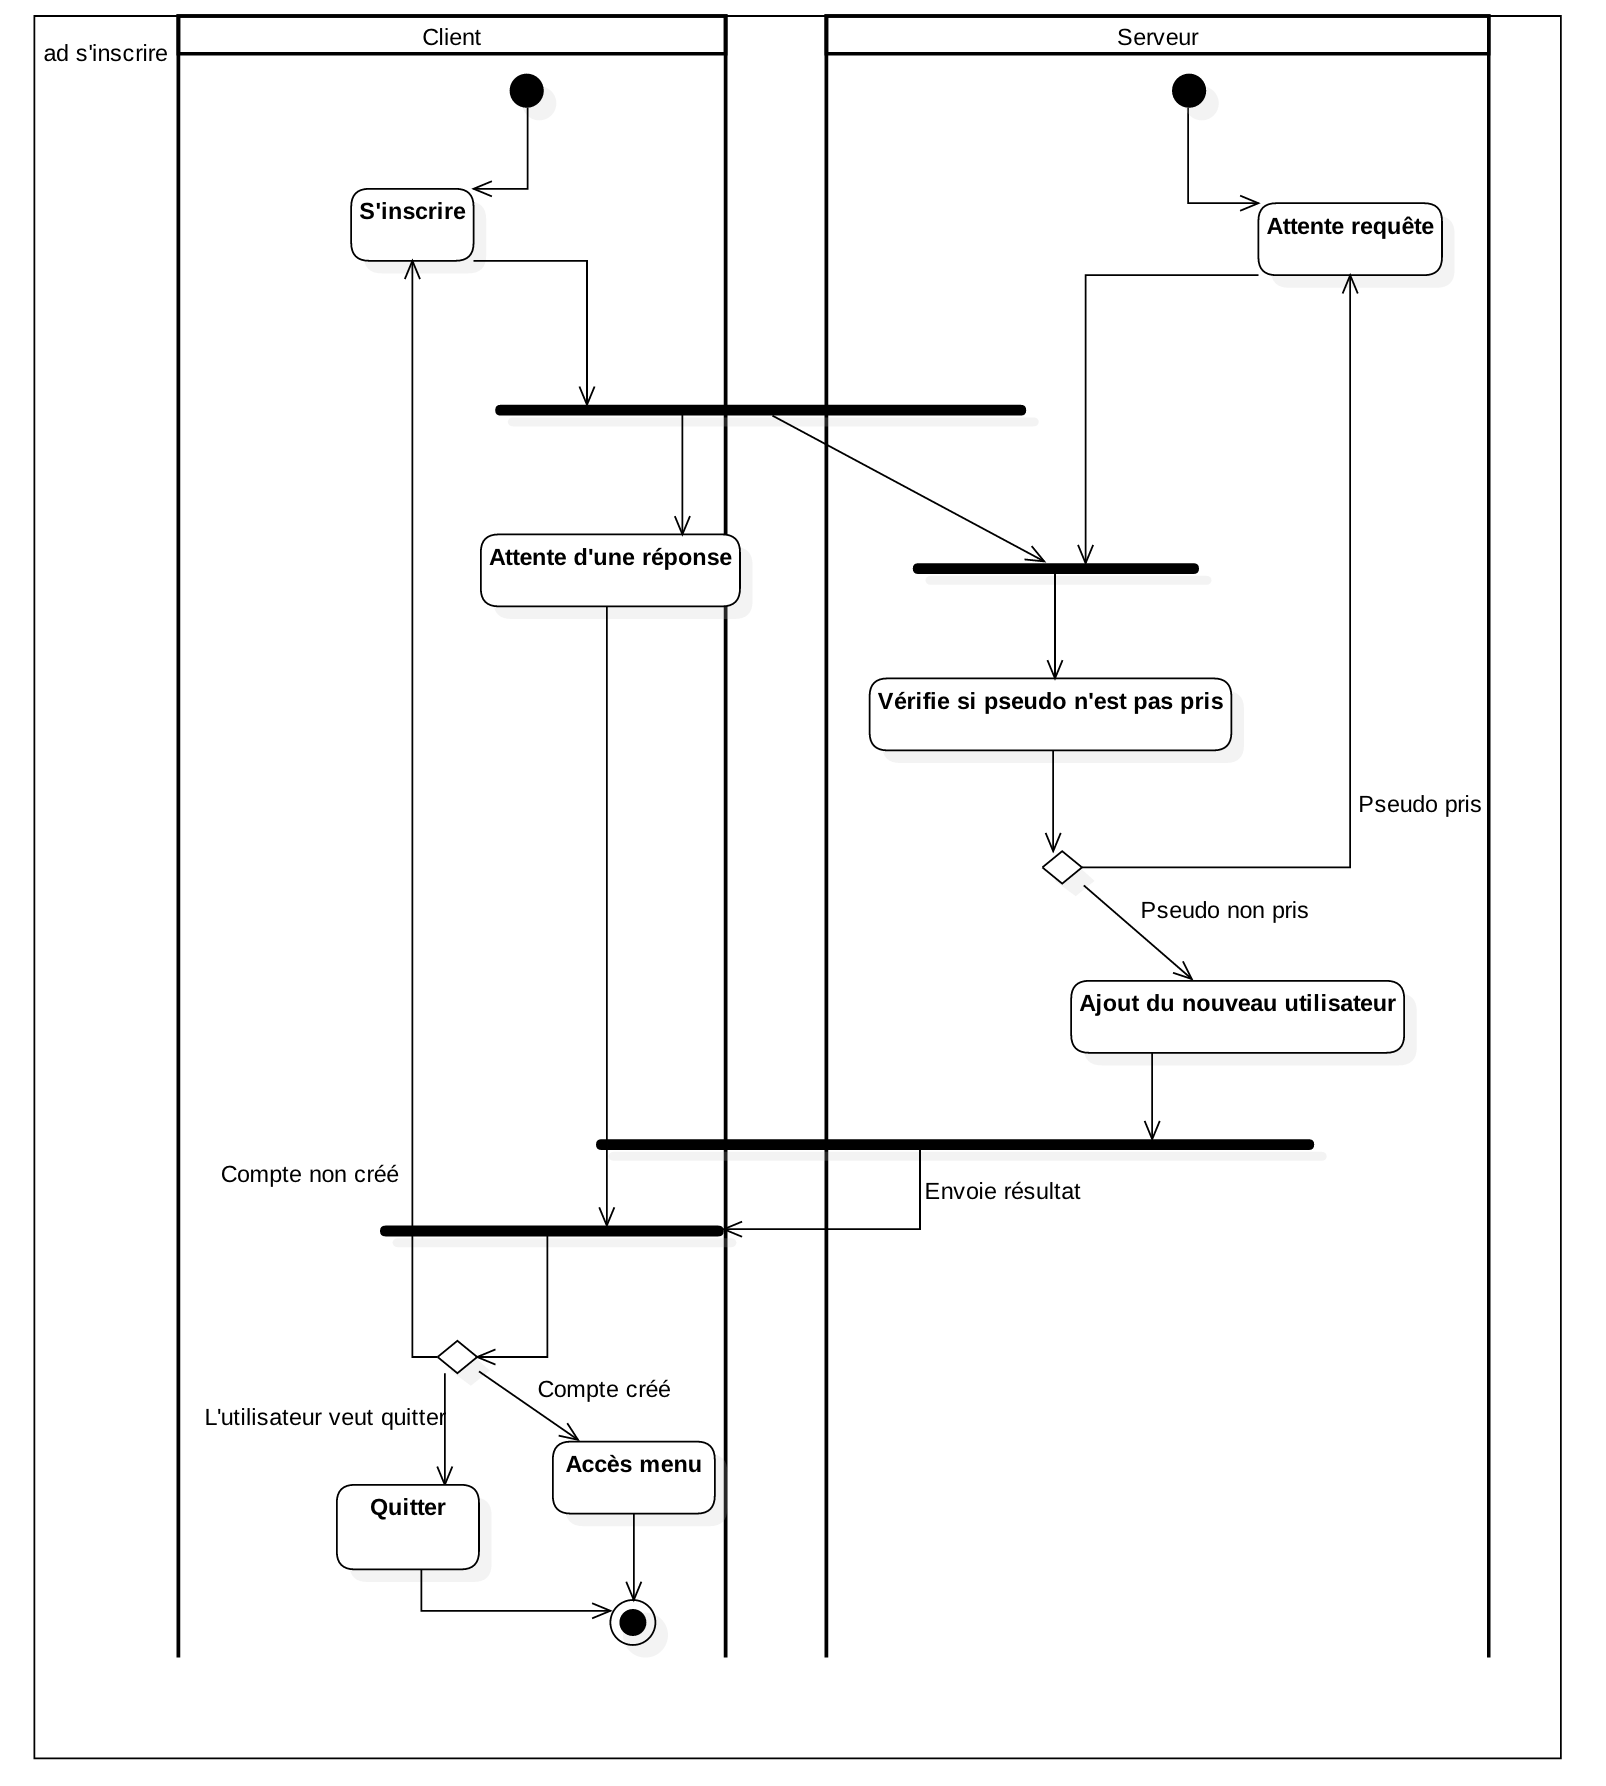
\includegraphics[height=18cm,width=18cm]{register.png}
    \caption{Diagramme d'activité inscription}
    \label{fig:picture}
 \end{figure}
\end{center}
\begin{center}
\begin{figure}[H]
    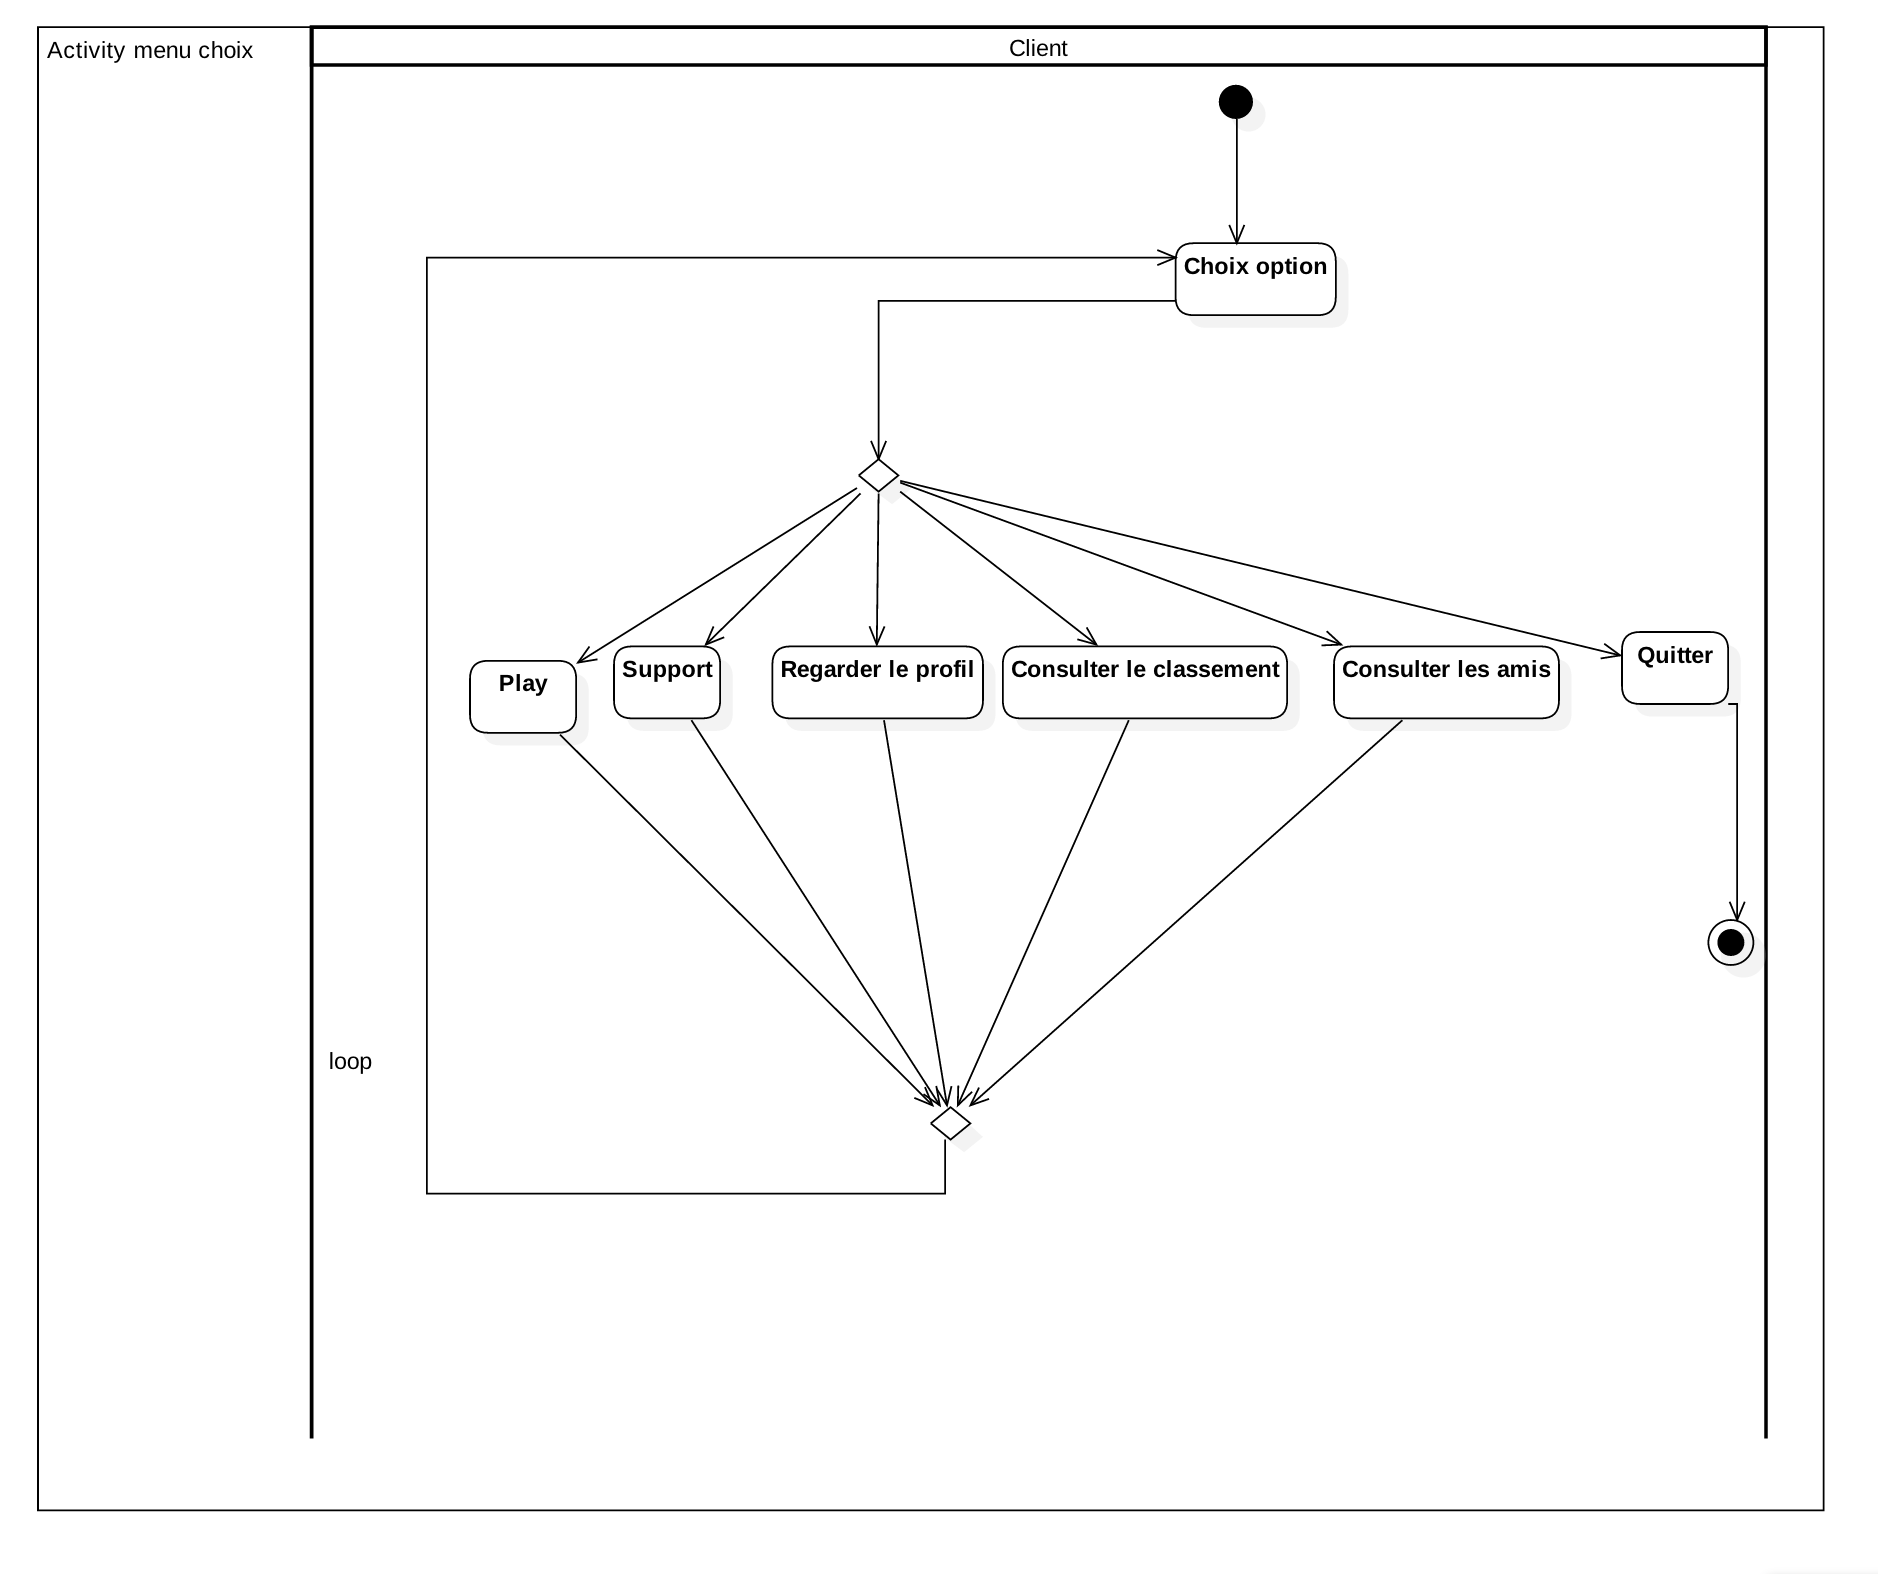
\includegraphics[height=18cm,width=18cm]{menuActi.png}
    \caption{Diagramme d'activité sur le menu}
    \label{fig:picture}
 \end{figure}
\end{center}
%\section{Index et termes utilisés}
\printindex

\end{document}
